\documentclass[a4paper,article,14pt]{extarticle}

% Подключаем главный пакет со всем необходимым
\usepackage{spbudiploma}

% Пакеты по желанию (самые распространенные)
% Хитрые мат. символы
\usepackage{euscript}
% Таблицы
\usepackage{longtable}
\usepackage{makecell}
% Картинки (можно вставлять даже pdf)
\usepackage[pdftex]{graphicx}

\usepackage{amsthm,amssymb,amsmath}
\usepackage{textcomp}

\usepackage{minted} % для примеров кода (требует параметра -shell-escape)
\usemintedstyle{tango}
\renewcommand{\theFancyVerbLine}{\normalsize \arabic{FancyVerbLine}}
\usepackage{listings}

\usepackage{comment}

% ===============================================

\renewcommand{\le}{\leqslant}
\renewcommand{\ge}{\geqslant}

\newcommand{\fakesc}[1]{\uppercase{{\footnotesize #1}}}
\renewcommand{\textsc}{\fakesc}

% ===============================================


\begin{document}

% Титульник в файле titlepage.tex
\newgeometry{left=30mm, top=20mm, right=15mm, bottom=20mm, nohead, nofoot}
\begin{titlepage}
\begin{center}

\textbf{Санкт--Петербургский государственный университет}\\
\textbf{Факультет математики и компьютерных наук}


\vspace{35mm}

\textbf{\textit{\large Остапенко Степан Сергеевич}} \\[8mm]
% Название
\textbf{\large Выпускная квалификационная работа}\\[3mm]
\textbf{\textit{\large Проверка выполнимости SMT-формул\\с помощью нейронных сетей}}

\vspace{20mm}
Уровень образования: бакалавриат\\
Направление 01.03.02 «Прикладная математика и информатика»\\
Основная образовательная программа СВ.5156.2020\\
«Современное программирование»\\[15mm]

% Научный руководитель, рецензент
\begin{flushright}
\begin{minipage}[t]{0.55\textwidth}
{Научный руководитель:} \\
доцент, \\
Факультет математики и \\
компьютерных наук СПбГУ, \\
к.ф.-м.н. Шалымов Дмитрий Сергеевич

\vspace{10mm}

{Рецензент:} \\
ведущий инженер ключевых проектов, \\
ООО «Техкомпания Хуавэй», \\
Ковальчук Сергей Валерьевич
\end{minipage}
\end{flushright}

\vspace{8mm}

{Санкт-Петербург}
\par{\the\year{} г.}
\end{center}
\end{titlepage}
\restoregeometry
\addtocounter{page}{1}


% Содержание
\tableofcontents
\pagebreak

% Также существуют особые главы - это
% "Введение",
% "Постановка задачи",
% "Обзор литературы",
% "Выводы",
% "Заключение".
% Они обязательно присутствуют, не нумеруются и должны идти в том порядке, в каком они идут в примере. 

\specialsection{Введение}

Введение широко представляет предметную область работы, указывает на место работы в научном или технологическом контексте.

\specialsection{Постановка задачи}

В постановке задачи коротко (по пунктам) указывается, что необходимо сделать в рамках работы.


\specialsection{Обзор литературы и предметной области}

Тема применения нейронных сетей в контексте решения формально-логических задач развита не особо сильно, поскольку дискретные задачи со строгими ограничениями тяжело даются сетям с известными на данный момент архитектурами. Тем не менее, известны многочисленные попытки использовать нейросети в качестве помощника для алгоритма, решающего ту или иную задачу. Про несколько таких подходов, имеющих отношение к проверке выполнимости и поиску решения для SMT-формул, я расскажу далее. Но перед этим я детально опишу устройство и архитектуру графовых нейронных сетей, поскольку на использовании данной архитектуры в значительной части основана моя работа.

\specialsubsection{Устройство GNN} \label{gnn-architecture}

Графовые нейронные сети\footnote{Далее по тексту будем называть их GNN (англ. \textit{Graph Neural Networks}).}, наряду со свёрточными, рекуррентными и т. д., являются одним из способов решать задачу машинного обучения, учитывая специфику данных. Так как графы отображают взаимоотношения между объектами некоторого множества, то и процесс построения модели, в данном случае, учитывает локальность и связи между произвольными объектами из предметной области.

Впервые архитектура GNN в общем виде была описана ещё в 2009 году в статье \cite{gnn-intro-paper}, однако широкую известность получила только в 2017 году после её применения для предсказания квантовых чисел в вычислительной органической химии \cite{gnn-quantum-chemistry-paper}. В основе вычислений лежит процесс \textit{передачи сообщений} между вершинами графа, который изображён\footnote{Подобное вычисление происходит для каждой вершины на каждой итерации процесса \textit{передачи сообщений}.} на рис.~\ref{message-passing-nn-architecture}: в каждой вершине хранится вектор-состояние (эмбеддинг\footnote{От англ. \textit{embedding} --- в машинном обучении так называют представление некоторого объекта в многомерном векторном пространстве.}), и на каждом шаге все вершины сначала рассылают свой текущий вектор всем своим непосредственным соседям, а потом агрегируют пришедшие от соседей векторы (\textit{сообщения}) и обновляют свой вектор-состояние с учётом этого; далее эти шаги повторяются несколько раз, после чего полученные таким образом векторы-состояния используются для построения представления графа и дальнейшего решения задачи.

% todo: написать, что вектор, состояние и эмбеддинг -- это одно и то же

\begin{figure}[ht]
\begin{center}
    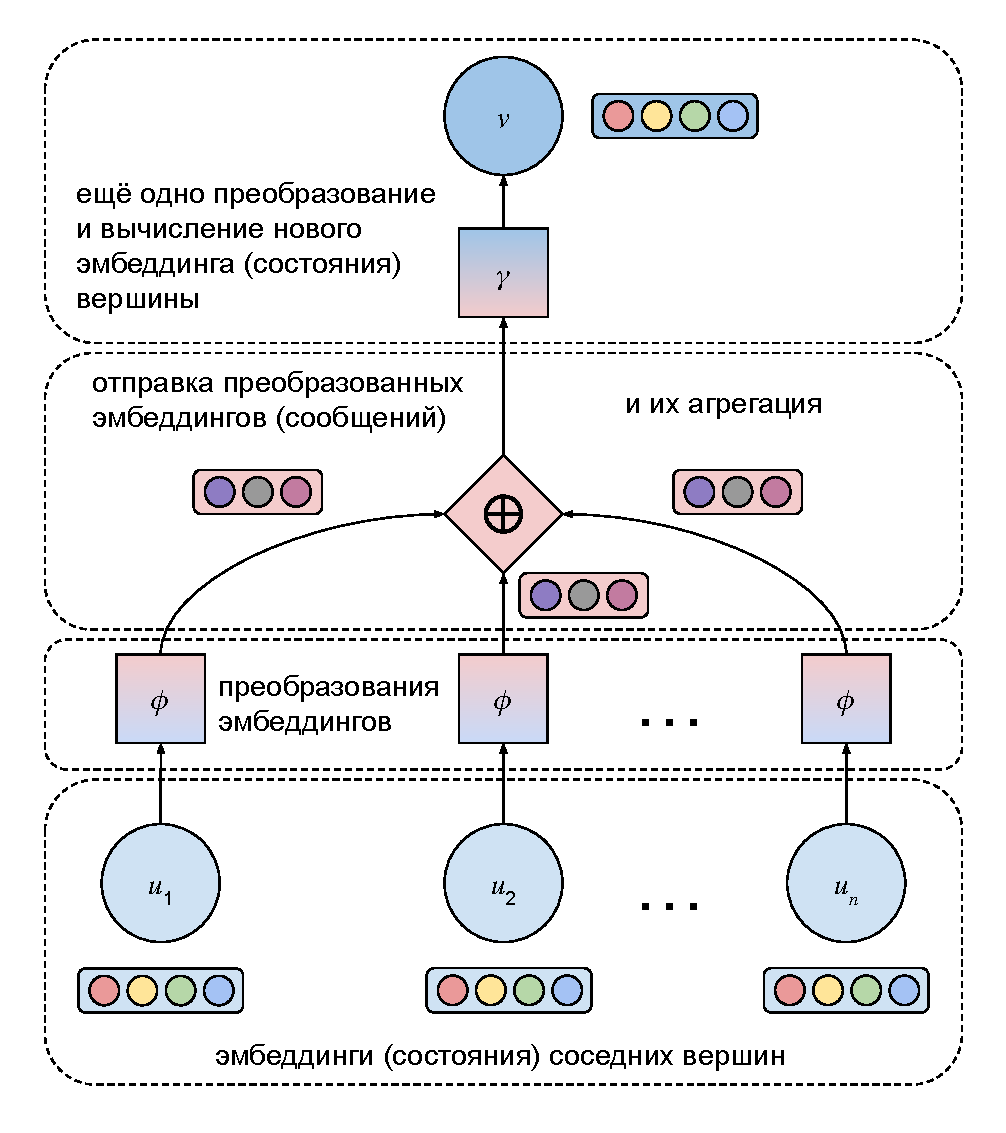
\includegraphics[scale=0.75]{./assets/message-passing-nn-architecture.pdf}
    \caption{\label{message-passing-nn-architecture} Схема обновления вектора-состояния вершины $v$ через векторы-сообщения от её соседей $u_1$, $u_2$, \ldots, $u_n$. Цвет (синий / красный) обозначает размерность. Более тёмный цвет вверху обозначает обновлённое состояние.}
\end{center}
\end{figure}

Согласно \cite{gnn-deep-learning-5g}, формально весь процесс устроен следующим образом:

\begin{itemize}
    \item у каждого ребра $e$ есть набор параметров $s_e \in \mathbb{R}^m$;
    \item в начале вычислений в каждой вершине $v$ содержится содержится вектор (состояние) $x_v^{(0)} \in \mathbb{R}^n$ с некоторой информацией;
    \item производится несколько итераций \textit{передачи сообщений}, на $t$-й из них производится обновление векторов в вершинах по правилу, которое описывается формулой~(\ref{gnn-state-update-rule});
    \item после всех итераций предполагается, что вычисленные векторы (состояния) образуют некоторое представление вершины / графа, поэтому их можно использовать в качестве параметров\footnote{Будем также называть их признаками или фичами (от англ. \textit{feature}).} вершины / графа, подавая в какую-нибудь MLP\footnote{Многослойный перцептрон (от англ. \textit{Multi-Layer Perceptron}) --- последовательная комбинация из полносвязных линейных слоёв и нелинейных слоёв активации.}-сеть.
\end{itemize}

\begin{equation} \label{gnn-state-update-rule}
    x_v^{(t)} = \gamma^{(t)} \left(x_v^{(t - 1)}, \bigoplus_{u \in \mathcal{N}(v)} \phi^{(t)} \left(x_v^{(t - 1)}, x_u^{(t - 1)}, s_{e(u \, \to \, v)} \right) \right)
\end{equation}

Обозначения в формуле~(\ref{gnn-state-update-rule}):

\begin{itemize}
    \item $x_v^{(t)} \in \mathbb{R}^n$ --- описанные выше эмбеддинги вершин;
    \item $e(u \, \to \, v)$ --- ребро из вершины $u$ в вершину $v$, а $s_{e(u \, \to \, v)} \in \mathbb{R}^m$ --- его параметры;
    \item $\mathcal{N}(v)$ --- окрестность вершины $v$;
    \item $\phi^{(t)}: \mathbb{R}^n \times \mathbb{R}^n \times \mathbb{R}^m \to \mathbb{R}^k$ --- функция создания сообщения по состояниям вершин и параметрам ребра; может быть представлена аффинным преобразованием, композицией линейных слоёв и нелинейных активаций, какими-нибудь сложными LSTM\footnote{Долгая краткосрочная память (от англ. \textit{Long Short-Term Memory}) --- известная модификация рекуррентной нейронной сети.} или GRU\footnote{Управляемый рекуррентный блок (от англ. \textit{Gated Recurrent Unit}) --- ещё одна известная модификация рекуррентной нейронной сети.}-слоями или просто любым дифференцируемым преобразованием с обучаемыми или необучаемыми параметрами;
    \item $\bigoplus: \mathbb{R}^k \to \mathbb{R}^k$ --- функция агрегации, например: сумма, среднее или взвешенная сумма с учётом механизма внимания;
    \item $\gamma^{(t)}: \mathbb{R}^n \times \mathbb{R}^k \to \mathbb{R}^n$ --- функция обновления вектора-состояния (эмбеддинга) вершины; аналогична $\phi^{(t)}$.
\end{itemize}

В качестве примера построения сети по такой схеме можно рассмотреть Graph Convolutional Network \cite{gcn-conv-paper}, самую популярную GNN-архитектуру. В её случае мы имеем:

\begin{itemize}
    \item $\phi^{(t)} = W^T \cdot x_u^{(t - 1)}$;
    \item $\bigoplus = \sum \limits_{u \in \mathcal{N}(v) \cup \{v\}} \dfrac{1}{\sqrt{|\mathcal{N}(v)|} \cdot \sqrt{|\mathcal{N}(u)|}} \cdot \phi^{(t)} \left(x_v^{(t - 1)}, x_u^{(t - 1)}, s_{e(u \, \to \, v)} \right)$;
    \item $\gamma^{(t)} = \bigoplus \limits_{u \in \mathcal{N}(v)} \phi^{(t)} \left(x_v^{(t - 1)}, x_u^{(t - 1)}, s_{e(u \, \to \, v)} \right) + b$;
\end{itemize}

\noindent где матрица весов $W$ и вектор-сдвиг $b$ являются выучиваемыми параметрами. Итого получаем:

\begin{equation}
    x_v^{(t)} = \sum \limits_{u \in \mathcal{N}(v) \cup \{v\}} \dfrac{1}{\sqrt{|\mathcal{N}(v)|} \cdot \sqrt{|\mathcal{N}(u)|}} \cdot \left(W^T \cdot x_u^{(t - 1)} \right) + b
\end{equation}

В настоящий момент GNN широко применяются для решения задач вычислительной физики, химии и биологии, построения рекомендательных систем, прогнозирования трафика на дорогах, распознавания объектов, синтеза текстов и речи \cite{gnn-global-overview} \cite{gnn-deep-learning-5g}.

% todo: написать, что такая штука совмещает в себе CNN и RNN

\specialsubsection{FastSMT}

В статье \cite{fastsmt-paper} рассматривается идея повышения эффективности SMT-решателя за счёт оптимизации его работы на формулах, возникающих в задачах из фиксированной предметной области.

Решатель в процессе своей работы применяет к формуле большое количество разных семантически эквивалентных преобразований\footnote{В статьях и документациях их называют тактиками.}, чтобы привести её к некоторому удобному для себя виду, в котором он сможет либо достаточно быстро найти решение для формулы и доказать, что оно подходит (тем самым доказав, что формула является выполнимой), либо достаточно быстро доказать, что указанный в формуле набор ограничений невозможно выполнить, и формула является невыполнимой. Примеры тактик: замена переменной, нормализация границ неравенства, bit-blasting (представление переменной в виде набора пропозициональных значений), переписывание условного оператора через конъюнкцию импликаций и т. д.. Упомянутый ранее решатель Z3 \cite{z3-paper} поддерживает более ста подобных операций.

Цепочка преобразований, которые решатель производит над формулой, формируется согласно некоторой стратегии, которая учитывает самые разнообразные параметры (признаки) формулы: от её размера и количества свободных переменных до некоторого приближения абстрактно-синтаксического дерева формулы. Сама стратегия, в данном случае, больше всего похожа на решающее дерево, у которого в вершинах стоят ограничения на очередные параметры формулы, а в каждом листе находится тактика, которую стоит применить в случае, когда параметры соответствуют пути в этот лист.

Базовую стратегию, которая используется в решателе по-умолчанию, подбирают его создатели, причём они делают это так, чтобы его средняя скорость работы на произвольной формуле была как можно лучше. В результате, решатель работает более стабильно (т. е. реже уходит в экспоненциальный перебор возможных решений, когда на вход подают сложную формулу), но скорость нахождения ответа в более простых случаях из-за этого проседает.

В то же время, большинство популярных современных инструментов для решения SMT-формул поддерживают возможность использования специфических стратегий, которые можно построить, в том числе, самостоятельно. Помимо этого, есть некоторая интуиция, что если мы будем рассматривать только формулы из некоторой фиксированной практической задачи, то все эти формулы будут обладать некоторой спецификой, знание о которой сможет существенно помочь в проверке их выполнимости. На этой интуиции, а также на возможности использовать собственные стратегии при решении формул строится подход, описанный в рассматриваемой статье.

Главная идея состоит в следующем: набор признаков формулы можно рассматривать как состояние некоторой среды, применение очередной тактики можно рассматривать как некоторое действие, совершаемое в этой среде, а награду за последовательность применённых тактик можно определить как суммарное время работы решателя на заданной формуле с использованием этой последовательности (разумеется, взятое с минусом), либо какому-нибудь штрафному значению в случае, если решатель не справляется с формулой. Таким образом, задача поиска оптимальной стратегии применения различных тактик хорошо представляется в виде задачи обучения с подкреплением, где средой является произвольная формула из некоторой фиксированной задачи. Поэтому предлагается выучивать модель (политику), которая по текущему состоянию среды (формулы) будет выдавать оптимальную тактику и параметры для неё.

\begin{figure}[ht]
\begin{center}
    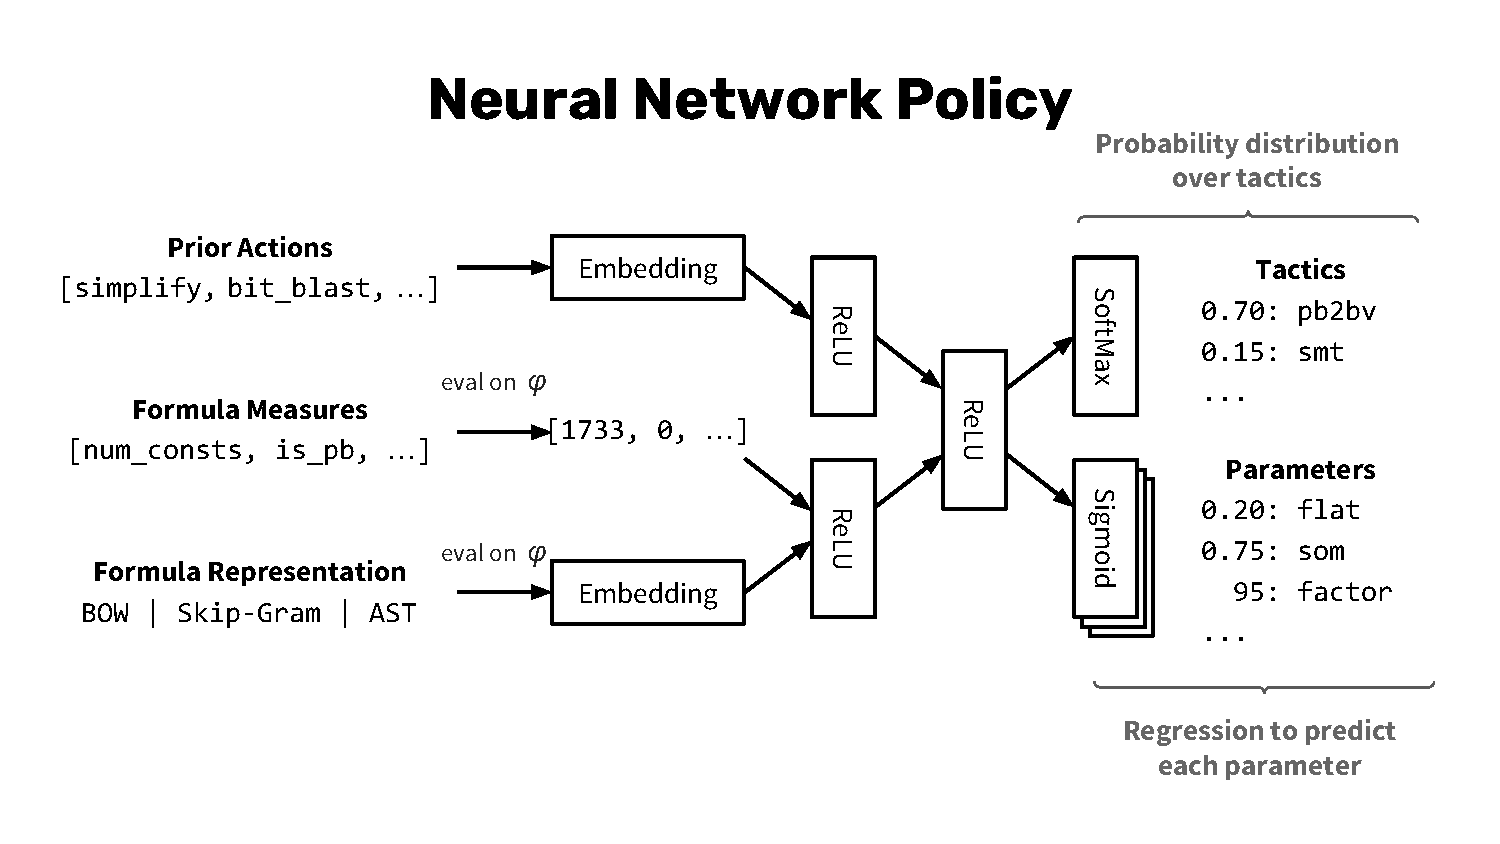
\includegraphics[scale=0.65]{./assets/fastsmt-nn-policy.pdf}
    \caption{\label{fastsmt-architecture} Архитектура модели. Картинка взята из статьи \cite{fastsmt-paper}.}
\end{center}
\end{figure}

Архитектура модели изображена на рис.~\ref{fastsmt-architecture}. На вход подаются признаки формулы (Formula Measures) и её синтаксическое представление, закодированное в виде bag-of-words или $n$-граммной модели (Formula Representation). Вдобавок к этому, для каждой тактики выучивается эмбеддинг, который хранит в себе семантическую информацию про неё. Эмбеддинги тактик, которые можно применить в данный момент, также подаются на вход модели (Prior Actions). На выходе у модели распределение на тактиках, которые стоит применить в данный момент, и значения параметров для них. Сразу отмечу, что, несмотря на то, что модель выдаёт распределение на всех доступных для применения в данный момент тактиках, за одно действие применяется только одна из них --- наиболее вероятная.

Построенная таким образом модель обучается на наборе формул взятом из некоторой задачи (в статье это были различные известные бенчмарки для решателей, на каждом из которых обучалась и оценивалась отдельная модель) с помощью метода, похожего на кросс-энтропийный метод. После этого с помощью техник семплирования строятся разнообразные статистики, отражающие выученную моделью политику, а уже на них обучается решающее дерево, выбирающее нужную тактику по текущей формуле, которое впоследствии превращается в стратегию, которую можно загрузить в SMT-решатель.

Авторы статьи заявляют, что, согласно проведённым экспериментам, предложенный подход позволяет успешно решать на 17\% больше формул при десятисекундном ограничении по времени, а также даёт прирост производительности вплоть до стократного ускорения на некоторых формулах (при этом, замедления при решении других формул не наблюдается). Тем не менее, у такого подхода есть существенный недостаток: для каждой новой задачи нужно сначала самостоятельно собирать данные, потом запускать тяжеловесный процесс обучения, а после этого самому синтезировать стратегию. Это требует довольно больших вычислительных мощностей.

\specialsubsection{GNN for Scheduling of SMT Solvers} \label{gnn-for-scheduling-of-smt-solvers}

В статье \cite{gnn-for-scheduling-paper} рассматривается более общий подход к задаче: известно, что в основе работы разных SMT-решателей лежат разные алгоритмы и эвристики, поэтому их производительность при решении разных формул может значительно варьироваться; в связи с этим, давайте просто обучим модель, которая по формуле будет предсказывать, за какое время тот или иной решатель сможет проверить её на выполнимость, а далее перед каждой проверкой будем выбирать решатель, для которого модель предсказывает наименьшее время работы.

Данная статья интересна тем, что в ней рассматривается более точное представление формулы, подаваемой модели на вход. Вместо сбора разных статистик с формулы и превращения их в признаки авторы предлагают использовать графовую нейронную сеть (GNN), которая задействует абстрактно-синтаксическое дерево\footnote{Далее в тексте будет использоваться аббревиатура AST (англ. \textit{Abstract-Syntax Tree}).} формулы в качестве графа вычислений (рис.~\ref{gnn-for-scheduling-architecture}).

\begin{figure}[ht]
\begin{center}
    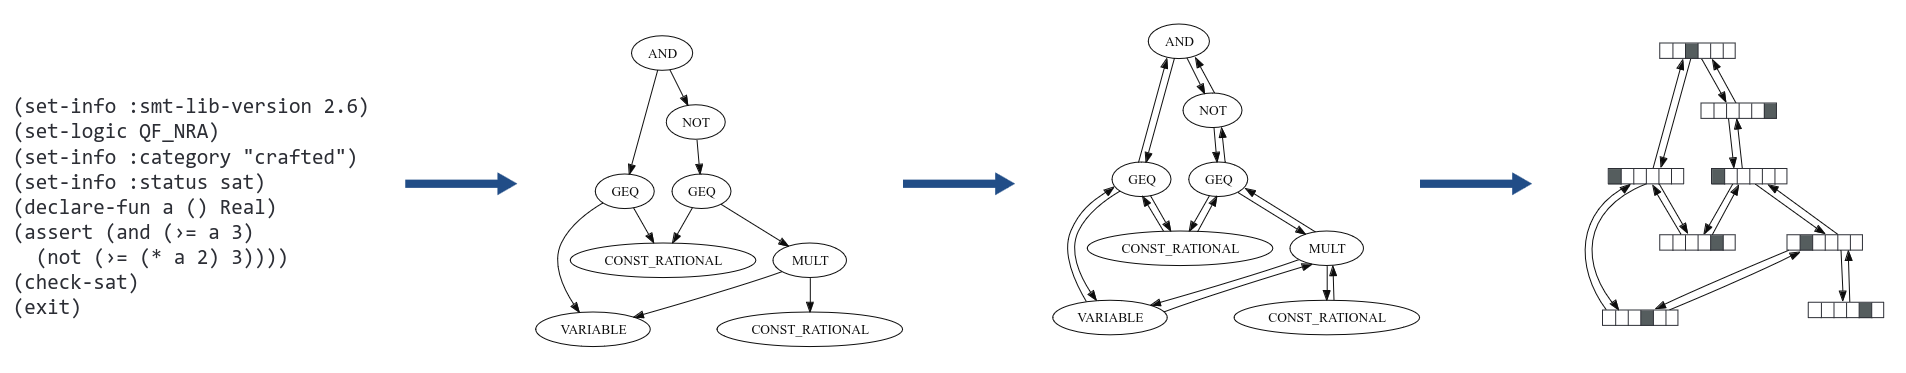
\includegraphics[scale=0.24]{./assets/gnn-for-scheduling-architecture.png}
    \caption{\label{gnn-for-scheduling-architecture} Использование AST формулы в качестве графа вычислений для GNN. Картинка взята из статьи \cite{gnn-for-scheduling-paper}.}
\end{center}
\end{figure}

Чтобы ускорить работу, вершины дерева, отвечающие за эквивалентные выражения, склеиваются в одну, так что формула, на самом деле, превращается в ориентированный ациклический граф. Помимо этого, чтобы расширить распространение эмбеддинга с информацией, сохранённой в каждой вершине, к каждому ребру такого графа добавляется обратное ребро. Таким образом, информация начинает распространяться сразу во всех направлениях.

\begin{figure}[ht]
\begin{center}
    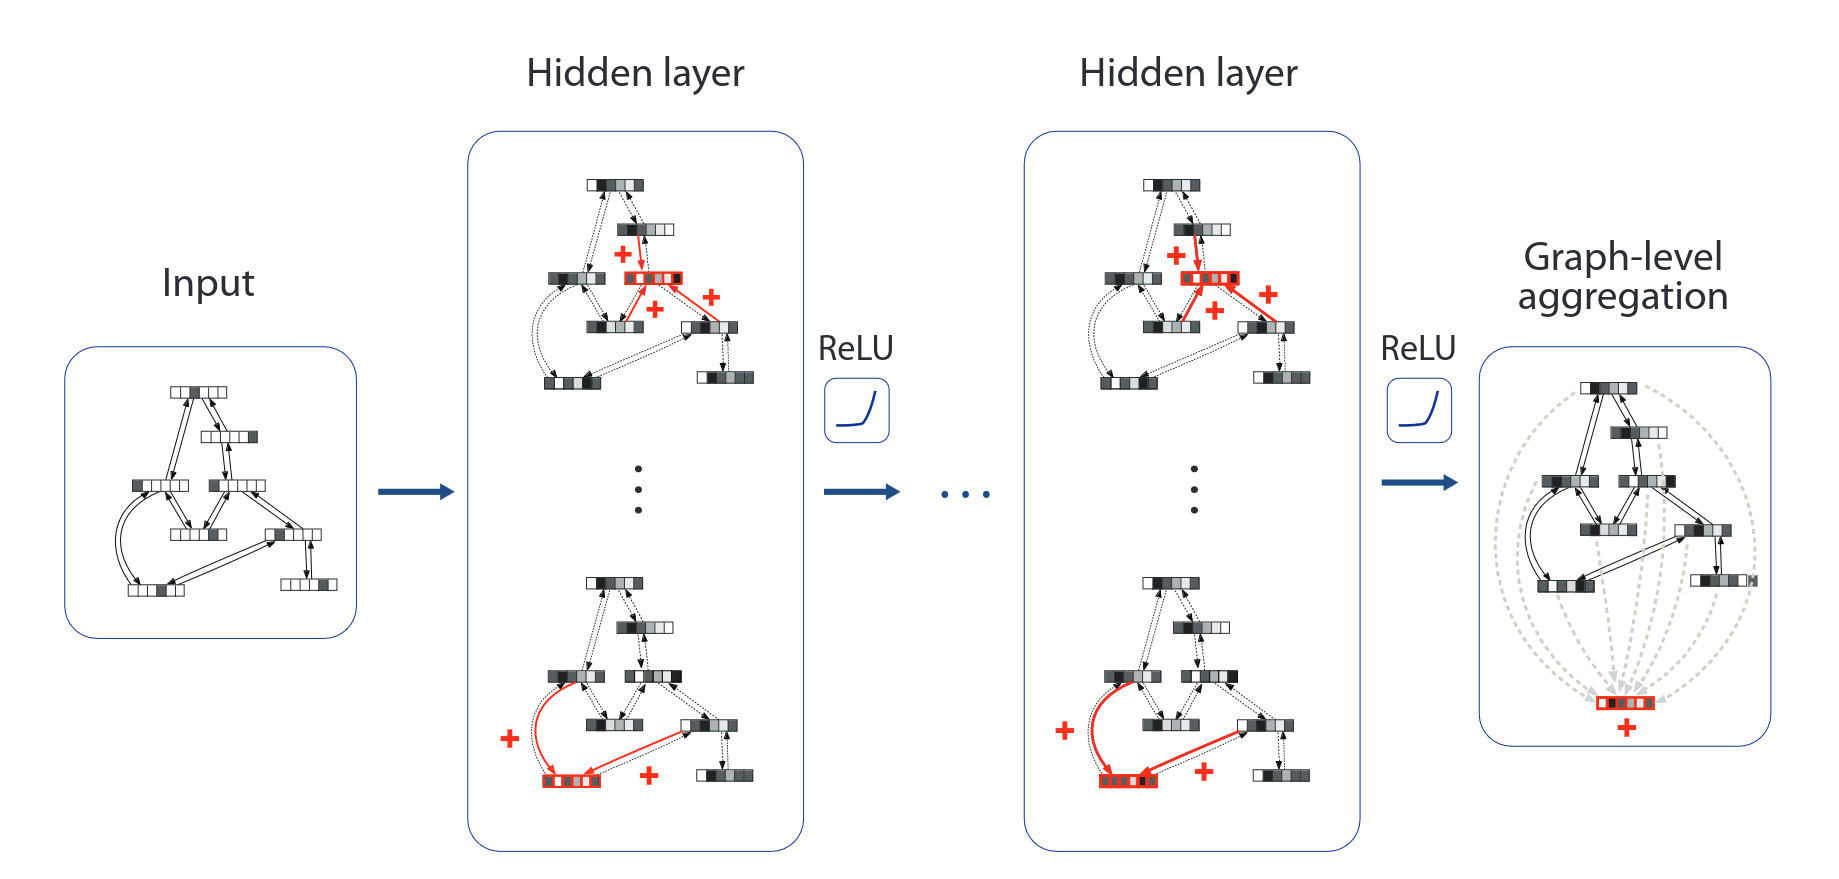
\includegraphics[scale=0.25]{./assets/gnn-for-scheduling-process.png}
    \caption{\label{gnn-for-scheduling-process} Схема использования GNN для получения информации о формуле и предсказания ответа. Картинка взята из статьи \cite{gnn-for-scheduling-paper}.}
\end{center}
\end{figure}

Далее каждая вершина (переменная, константа или операция) кодируется с помощью техники one-hot-encoding, после чего векторы с полученными таким образом значениями отправляются в GNN, на выходе у которой находится слой, собирающий эмбеддинги со всех вершин графа и предсказывающий для каждого SMT-решателя время, за которое он может выдать ответ на данной формуле. Для лучшего понимания, схема процесса изображена на рис~\ref{gnn-for-scheduling-process}.

Авторы отмечают, что подход может быть применён для решения почти для любой SMT-формулы, и утверждают, что им удалось добиться ускорения процесса на 8--900\% на разных тестах.

\specialsubsection{NeuroSAT}

Тем не менее, попытки научиться решать формально-логическую задачу, пользуясь исключительно нейронными сетями, тоже присутствуют. Пионером в этой области стала работа \cite{neurosat-paper}, в которой исследовалось применение GNN для задачи SAT. Была предложена следующая графовая архитектура: для каждой переменной, для отрицания каждой переменной и для каждого конъюнкта формулы заводится по вершине; далее рёбра проводятся между парами из литерала (переменными или их отрицаниями) и конъюнкта, если литерал входит в состав конъюнкта, а также между парами противоположных литералов (теми, которые является отрицаниями друг друга). Пример построения такого графа изображён на рис.~\ref{neurosat-mpnn}.

\begin{figure}[ht]
\begin{center}
    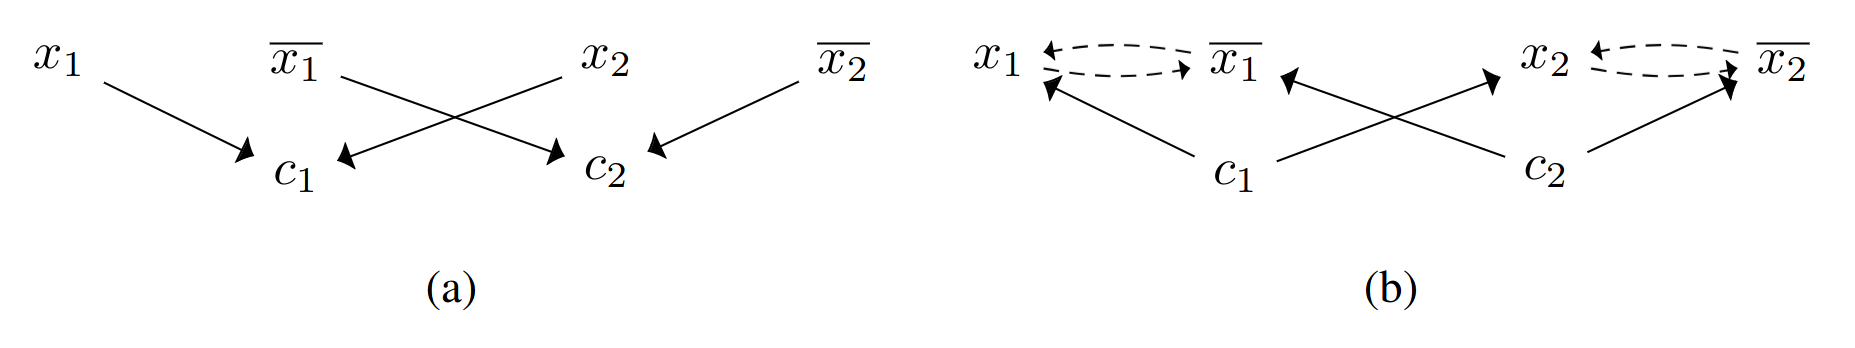
\includegraphics[scale=0.25]{./assets/neurosat-mpnn.png}
    \caption{\label{neurosat-mpnn} Граф, построенный для формулы $(x_1 \vee x_2) \wedge (\overline{x_1} \vee \overline{x_2})$. Пункты (a) и (b) отражают шаги построения, описанные в статье; на деле же граф выглядит как их объединение. Картинка взята из статьи \cite{neurosat-paper}.}
\end{center}
\end{figure}

Во время вычислений каждая вершина накапливает все пришедшие к ней сообщения с помощью LSTM-слоя. После каждого шага передачи сообщений по графу каждая вершина-литерал генерирует собственное предсказание по поводу того, является ли данная формула выполнимой (внутреннее состояние LSTM отправляется в многослойный классификатор (MLP), который предсказывает одно число --- степень уверенности вершины в том, что формула выполнима).

\begin{figure}[ht]
\begin{center}
    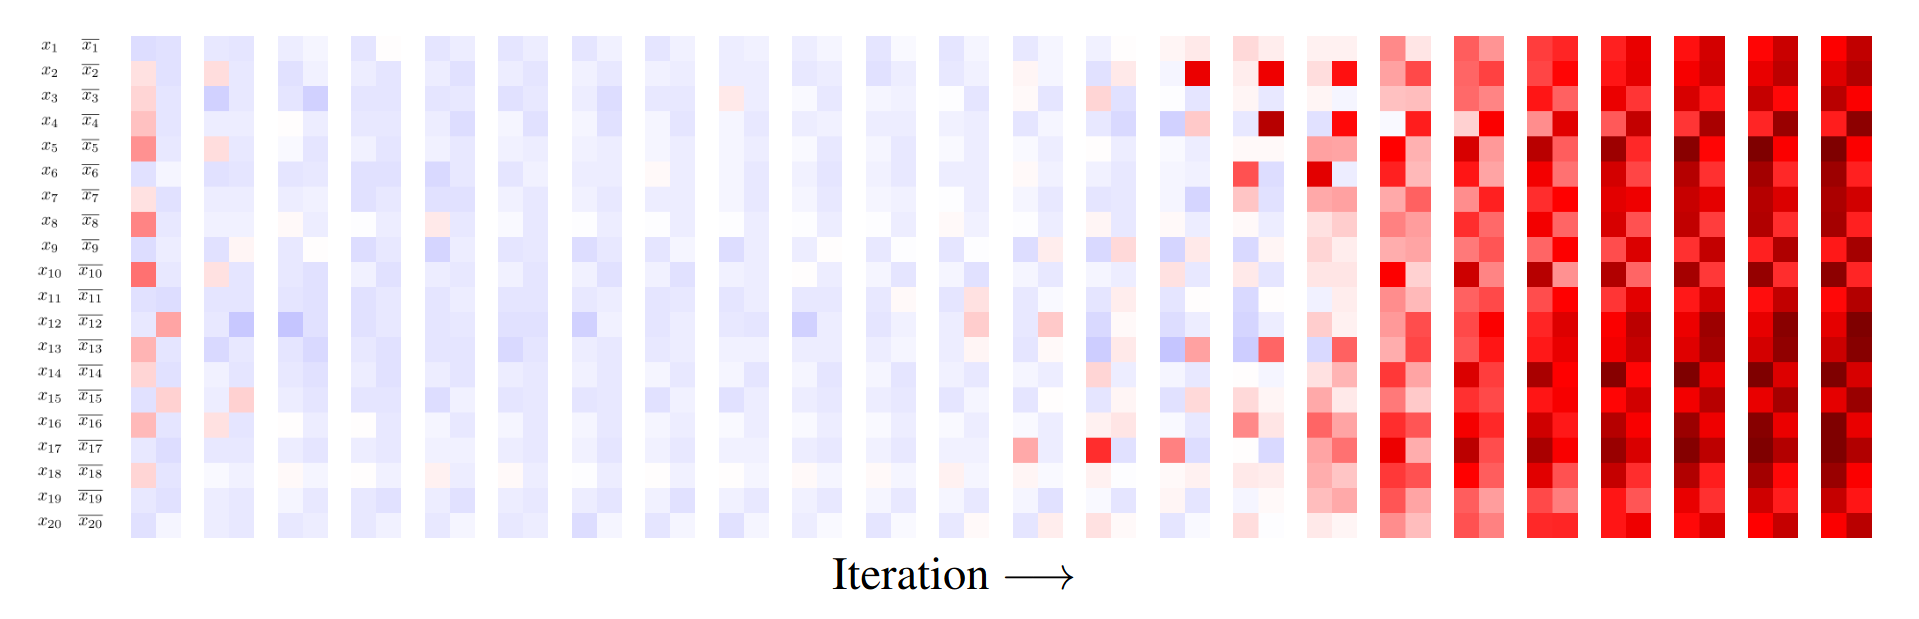
\includegraphics[scale=0.24]{./assets/neurosat-voting.png}
    \caption{\label{neurosat-voting} Граф, построенный для формулы $(x_1 \vee x_2) \wedge (\overline{x_1} \vee \overline{x_2})$. Пункты (a) и (b) отражают шаги построения, описанные в статье; на деле же граф выглядит как их объединение. Картинка взята из статьи \cite{neurosat-paper}.}
\end{center}
\end{figure}

% todo: дописать neurosat

% эмбеддинги
% дописать про GatedGraphConv https://pytorch-geometric.readthedocs.io/en/latest/generated/torch_geometric.nn.conv.GatedGraphConv.html#torch_geometric.nn.conv.GatedGraphConv
% слой голосования
% итерации
% результаты
% случайные формулы

% \hrule

% todo: дописать про другие работы
% \specialsubsection{Другие работы}

% mach smt
% alpha geometry
% Learning the Satisfiability of Pseudo-Boolean Problem with Graph Neural Networks
% https://ruoyuwang.me/bar2019/pdfs/bar2019-final80.pdf
% https://www.semanticscholar.org/paper/Algorithm-selection-for-SMT-Scott-Niemetz/aff1afe03f8e2f636b972add9b03ac59f6c34223
% https://www.semanticscholar.org/paper/On-EDA-Driven-Learning-for-SAT-Solving-Li-Shi/5c4bb681fe5cb159b0d577b784fa52c952871e17
% https://www.semanticscholar.org/paper/SATformer%3A-Transformer-Based-UNSAT-Core-Learning-Shi-Li/06547a615390ba14d37c684136c30a4ac559d610
% https://www.semanticscholar.org/paper/NeuroBack%3A-Improving-CDCL-SAT-Solving-using-Graph-Wang-Hu/a613142147ef740b2daf1265e23606c80d1c2bd2
% https://www.semanticscholar.org/paper/Synthesizing-Smart-Solving-Strategy-for-Symbolic-Chen-Chen/c7f8cd87ae269bb8b85eeb627005b7884a81bee0
% Combinatorial Optimization with Graph Convolutional Networks and Guided Tree Search https://arxiv.org/abs/1810.10659
% Andrew W Senior, Richard Evans, John Jumper, James Kirkpatrick, Laurent Sifre, Tim Green, Chongli Qin, Augustin Žídek, Alexander WR Nelson, Alex Bridgland, et al. Improved protein structure prediction using potentials from deep learning. Nature, 577(7792):706–710, 2020.


\section{Датасет} \label{datasets}

В своей работе я использовал два датасета с SMT-формулами:

\begin{enumerate}
    \item Бенчмарк\footnote{Набор данных для тестирования корректности или производительности программы.} с SMT-COMP 2023 \cite{smt-comp-2023-benchmarks}.
    \item Формулы, собранные в процессе работы дважды упомянутого выше символьного движка USVM \cite{usvm-diploma}.
\end{enumerate}

\subsection{SMT-COMP}

В процессе исследований этот бенчмарк был поделен на три части:

\begin{enumerate}
    \item \texttt{BitVec} --- формулы из логики \texttt{QF\_BV}, обычные формулы с битовыми векторами;
    \item \texttt{SymbEx} --- формулы из логик \texttt{QF\_BV}, \texttt{QF\_ABV}, \texttt{QF\_ABVFP}, \texttt{QF\_AUFBV}, \\ \texttt{QF\_AUFBVFP}, \texttt{QF\_BVFP}, \texttt{QF\_FP}, \texttt{QF\_UF}, \texttt{QF\_UFBV} и \texttt{QF\_UFFP}, которые возникают в процессе работы любого движка для символьного исполнения;
    \item \texttt{QuaFree} --- формулы из всех безкванторных логик, включая \texttt{QF\_LIA}, \texttt{QF\_NRA}, \texttt{QF\_BVFPLRA} и т. д..
\end{enumerate}

Такое разделение обусловлено тем, что для анализа качества хочется смотреть, как модель обучается и какое качество она выдаёт на формулах из разных логик. Однако, к сожалению, большинство логик в данном бенчмарке содержат слишком мало данных, чтобы можно было провести анализ на них, поэтому было принято решение объединить логики в группы по смыслу. Логика \texttt{QF\_BV} была вынесена в отдельную группу, поскольку она является самой многочисленной, а также самой важной на практике. Логики из группы \texttt{SymbEx} были собраны вместе, поскольку моя текущая задача существует в контексте символьного исполнения, поэтому хочется отдельно анализировать способность модели решать подобные формулы. В оставшуюся группу \texttt{QuaFree} попали все безкванторные логики, так как хочется также анализировать способность модели решать задачу в некотором общем случае. В дальнейшем каждую группу будем называть датасетом с соответствующим именем.

Формулы с кванторами в данной работе не рассматривались вообще, поскольку они существенно сложнее безкванторных, и их было решено отложить до лучших времён.

Чтобы данные влезли на видеокарту в каждом датасете были оставлены только формулы размером\footnote{Размером формулы считаем количество переменных, констант и операций в ней. Например, размер формулы $(x + y = 5) \vee (z = 3)$ равен 9.} не более 10\,000 и глубиной\footnote{Глубиной формулы считаем максимальную вложенность переменных, констант и операций в ней. Например, глубина формулы $(x + y = 5) \vee (z = 3)$ равна 4.} не более 2\,000. Итоговые параметры построенных датасетов отображены в таблице~\ref{smt-comp-datasets-table}.

\begin{table}[ht]
\begin{center}
\begin{tabular}{r|cccc}
    Датасет & \makecell{Количество \\ формул} & \makecell{Средний \\ размер \\ формулы} & \makecell{Средняя \\ глубина \\ формулы} & \makecell{Доля \\ выполнимых \\ формул} \\
    \hline \hline
    \rule{0pt}{2.5ex}
    \texttt{BitVec}  &  33\,797 & 1181.92 & 85.45 & 0.378 \\
    \texttt{SymbEx}  &  85\,078 &  669.46 & 49.24 & 0.610 \\
    \texttt{QuaFree} & 123\,396 &  965.16 & 48.71 & 0.622 \\
\end{tabular}
\caption{\label{smt-comp-datasets-table} Параметры датасетов, полученных из данных с SMT-COMP 2023 \cite{smt-comp-2023-benchmarks}.}
\end{center}
\end{table}

\subsection{USVM} \label{usvm-datasets-desc}

Для проверки возможности применения модели на практике были также собраны датасеты, состоящие из формул, которые возникают в процессе работы символьного движка USVM \cite{usvm-diploma}. Такая идея возникла, поскольку в статье \cite{fastsmt-paper}, описанной в разделе \underline{\hyperref[fastsmt]{FastSMT}}, было показано, что обучение модели на формулах, собранных с какой-то конкретной задачи, может помочь в решении других формул, возникающих в этой же самой задаче.

Сбор осуществлялся с помощью простого логирования формул, на которых вызывался SMT-решатель. Разные датасеты получались при запуске движка на разных проектах или наборах программ. Подобным образом были собраны три тренировочных и восемнадцать валидационных датасетов.

Такое строгое разделение на тренировочные и валидационные датасеты вдобавок к такому большому количеству вторых обусловлено желанием проверить обобщающую способность модели: хочется, чтобы модель показывала хорошее качество на формулах, возникающих при запуске движка на любых программах; при этом, нет никаких гарантий, что при переходе от одного набора программ к другому распределение, из которого порождаются формулы, изменится несущественно, и качество модели, обученной на данных из другого распределения, упадёт не слишком сильно.

Тренировочные датасеты были собраны на следующих программах:

\begin{enumerate}
    \item \texttt{usvm-test} --- на наборе программ для unit и интеграционного тестирования USVM;
    \item \texttt{the-algorithms} --- на репозитории с реализациями различных теоретических и практических алгоритмов на Java;
    \item \texttt{usvm-core} --- на ядре символьного движка USVM (движок был запущен на самом себе).
\end{enumerate}

Параметры тренировочных датасетов указаны в таблице~\ref{usvm-train-datasets-table}.

\begin{table}[ht]
\begin{center}
\begin{tabular}{r|cccc}
    Датасет & \makecell{Количество \\ формул} & \makecell{Средний \\ размер \\ формулы} & \makecell{Средняя \\ глубина \\ формулы} & \makecell{Доля \\ выполнимых \\ формул} \\
    \hline \hline
    \rule{0pt}{2.5ex}
    \texttt{usvm-test}      & 153\,778 & 522.84 &  5.18 & 0.038 \\
    \texttt{the-algorithms} & 181\,633 & 277.03 & 23.94 & 0.066 \\
    \texttt{usvm-core}      & 192\,744 & 179.42 & 12.19 & 0.066 \\
\end{tabular}
\caption{\label{usvm-train-datasets-table} Параметры тренировочных датасетов, собранных в процессе работы USVM.}
\end{center}
\end{table}

Валидационные датасеты были собраны при запуске USVM на следующих проектах, написанных на Java и других JVM-языках:

\begin{enumerate}
    \item \texttt{owasp} --- OWASP\footnote{Open Web Application Security Project.}, открытый бенчмарк из программ на Java, на котором оценивают качество инструментов для автоматического поиска уязвимостей в коде \cite{owasp-website};
    \item \texttt{cassandra} --- Apache Cassandra, распределённая NoSQL СУБД\footnote{Система Управления Базами Данных.} \cite{cassandra-website};
    \item \texttt{kafka} --- Apache Kafka, распределённый брокер сообщений \cite{kafka-website};
    \item \texttt{spark-core} --- Apache Spark, система для распределённой обработки данных (модуль ядра) \cite{spark-website};
    \item \texttt{spark-streaming} --- тот же Spark (модуль потоковой обработки данных);
    \item \texttt{utbot-core} --- UnitTestBot, инструмент для автоматической генерации unit-тестов (модуль ядра) \cite{utbot-github};
    \item \texttt{utbot-java} --- тот же UnitTestBot (модуль генерации тестов для Java);
    \item \texttt{utbot-python} --- тот же UnitTestBot (модуль генерации тестов для Python);
    \item \texttt{utbot-js} --- тот же UnitTestBot (модуль генерации тестов для языка JavaScript);
    \item \texttt{utbot-go} --- тот же UnitTestBot (модуль генерации тестов для Go);
    \item \texttt{zookeeper} --- Apache Zookeeper, служба для координации распределённых систем \cite{zookeeper-website};
    \item \texttt{elasticsearch} --- Elasticsearch, встраиваимая система для текстового поиска \cite{elasticsearch-website};
    \item \texttt{hbase} --- Apache HBase, распределённая табличная база данных \cite{hbase-website};
    \item \texttt{guava} --- Google Guava, набор библиотек-расширений для Java \cite{guava-website};
    \item \texttt{hadoop-common} --- Apache Hadoop, экосистема для распределённого хранения и обработки данных (модуль ядра) \cite{hadoop-website};
    \item \texttt{hadoop-hdfs} --- тот же Hadoop (модуль распределённой файловой системы);
    \item \texttt{hadoop-mapreduce} --- тот же Hadoop (модуль для распределённых вычислений в парадигме MapReduce);
    \item \texttt{hadoop-yarn} --- тот же Hadoop (модуль планировщика ресурсов);
\end{enumerate}

Параметры валидационных датасетов указаны в таблице~\ref{usvm-val-datasets-table}.

\begin{table}[ht]
\begin{center}
\begin{tabular}{r|cccc}
    Датасет & \makecell{Количество \\ формул} & \makecell{Средний \\ размер \\ формулы} & \makecell{Средняя \\ глубина \\ формулы} & \makecell{Доля \\ выполнимых \\ формул} \\
    \hline \hline
    \rule{0pt}{2.5ex}
    \texttt{owasp}            &  30\,935 & 3169.44 &  27.0  & 0.029 \\
    \texttt{cassandra}        &  13\,896 &  164.84 &  11.73 & 0.057 \\
    \texttt{kafka}            &  46\,867 & 5103.27 &  18.93 & 0.083 \\
    \texttt{spark-core}       &  14\,504 & 5599.33 &  28.0  & 0.061 \\
    \texttt{spark-streaming}  &  69\,254 & 1168.64 &  8.31  & 0.057 \\
    \texttt{utbot-core}       &  31\,043 & 4570.6  &  28.95 & 0.061 \\
    \texttt{utbot-java}       &  12\,492 &  116.4  &  10.71 & 0.045 \\
    \texttt{utbot-python}     &  24\,893 &  266.66 &  6.04  & 0.115 \\
    \texttt{utbot-js}         &  13\,276 & 2286.54 & 133.8  & 0.062 \\
    \texttt{utbot-go}         &  43\,988 &  281.69 &  19.21 & 0.014 \\
    \texttt{zookeeper}        &  38\,631 & 1196.51 &  47.23 & 0.046 \\
    \texttt{elasticsearch}    &  38\,967 &  388.62 &  19.72 & 0.001 \\
    \texttt{hbase}            &  38\,049 & 3513.78 &  90.81 & 0.019 \\
    \texttt{guava}            &  56\,607 &  545.98 &  34.99 & 0.014 \\
    \texttt{hadoop-common}    &  41\,255 &  419.05 &  10.32 & 0.081 \\
    \texttt{hadoop-hdfs}      & 109\,294 & 2795.7  & 210.87 & 0.032 \\
    \texttt{hadoop-mapreduce} &  12\,044 & 1294.2  &  47.17 & 0.011 \\
    \texttt{hadoop-yarn}      &  32\,555 &  120.71 &  13.01 & 0.035 \\
\end{tabular}
\caption{\label{usvm-val-datasets-table} Параметры валидационных датасетов, собранных в процессе работы USVM.}
\end{center}
\end{table}

Отмечу, что в валидационных датасетах также отобраны формулы, размер и глубина которых не превышает 10\,000 и 2\,000 соответственно, но, помимо этого, здесь добавилось ещё одно условие: размер должен быть не меньше некоторого значения, которое подбиралось эмпирическим путём отдельно для каждого датасета (обычно оно находилось в районе 200--500, и его можно угадать, если посмотреть на средний столбец в таблице). Поэтому формулы из валидационных датасетов кажутся больше, чем из тренировочных. Это было сделано, чтобы уменьшить объём данных и ускорить вычисления, а также чтобы оценивать качество модели именно на больших формулах, так как кажется, что на практике модель должна существенно помогать движку именно в этом случае.

Ещё внимательный читатель может заметить, что во всех датасетах из формул, собранных в процессе работы USVM, есть огромный дисбаланс классов: меньше десяти процентов формул являются выполнимыми. На самом деле, в этом нет ничего неожиданного, потому что в процессе символьного исполнения программы SMT-решателю действительно чаще всего приходится иметь дело с невыполнимыми формулами.

% todo: кажется, тут стоит ещё дописать

\subsection{Метрики}

Поскольку в работе рассматривается задача бинарной классификации, было принято решение следить за двумя метриками: ROC-AUC (площадь под ROC-кривой, далее будет обозначаться <<ROC-AUC>>) и Average Precision (площадь под precision-recall кривой, далее будет обозначаться <<AP>>) для случая, когда представителями положительного класса считаются выполнимые формулы. Пример на рис.~\ref{roc-auc-vs-au-prc}.

\begin{figure}[!ht]
\begin{center}
    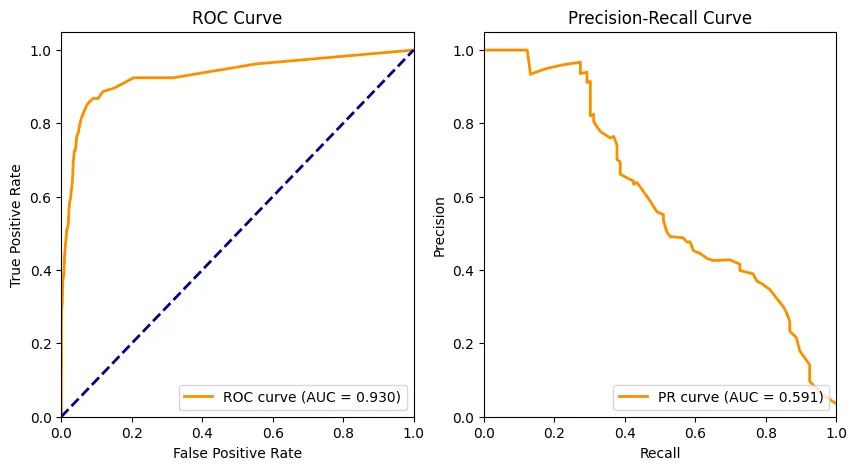
\includegraphics[scale=0.5]{./assets/roc-auc-vs-au-prc.jpg}
    \caption{\label{roc-auc-vs-au-prc} Пример вычисления ROC-AUC и AP. Источник: \url{https://juandelacalle.medium.com/how-and-why-i-switched-from-the-roc-curve-to-the-precision-recall-curve-to-analyze-my-imbalanced-6171da91c6b8} (дата обр. 27.05.2024).}
\end{center}
\end{figure}

Использование ROC-AUC обусловлено тем, что, помимо классификационной, это ещё и ранжирующая метрика, а в работе будет также интересно смотреть и на ранжирующие способности модели. Использование AP обусловлено тем, что ROC-AUC начинает терять репрезентативность, если в выборке данных появляется большой дисбаланс классов \cite{ap-vs-roc-auc-paper}.

Отмечу два факта, которые понадобятся в дальнейшем:

\begin{enumerate}
    \item ROC-AUC для случайного предсказания, а также для предсказания всем примерам положительной или предсказания всем примерам отрицательной метки равен $0.5 \pm \varepsilon$.
    \item AP для случайного предсказания, а также для предсказания всем примерам положительной или предсказания всем примерам отрицательной метки равен $t \pm \varepsilon$, где $t$ --- доля примеров положительного класса в выборке.
\end{enumerate}

Исходя из этого, можно для каждого датасета посчитать базовые значения метрик и сравнивать полученные результаты с ними, чтобы показать, что решение имеет хоть какой-то смысл.

Таким образом, в представленных результатах будет указано по два значения ROC-AUC и AP --- базовое, которое вычислено согласно только что изложенным фактам, и тестовое, которое получено при валидации обученной ранее модели на этом датасете. В таблицах с результатами базовое значение будет называться <<контрольным>>, а полученное при валидации --- <<тестовым>>. Выбранные названия отсылают к описанию результатов A/B-тестов (однако, это только отсылки --- в действительности, никакие A/B-тесты в данной работе не проводились).

Помимо этого, в одном из экспериментов будет считаться метрика <<precision at fixed recall>>, которая выражает уровень точности при заданном уровне полноты. За этими значениями тоже полезно следить, так как для символьного движка выполнимые формулы (которые в нашей задаче являются представителями положительного класса) гораздо интереснее, чем невыполнимые.

% todo: \section{Текстовый подход}

\newpage

\section{Подход с использованием GNN}

\subsection{Архитектура нейронной сети для решения задачи}

Придуманное в ходе работы решение объединяет в себе идеи из всех статей, рассмотренных в главе про обзор литературы и предметной области.

В качестве основной архитектуры для решения задачи была выбрана некоторая аппроксимация \underline{\hyperref[gnn-architecture]{GNN}}, работающая схожим образом с тем, что было ранее описано в разделе \underline{\hyperref[gnn-for-scheduling-of-smt-solvers]{GNN for Scheduling of SMT Solvers}} \cite{gnn-for-scheduling-paper}, и заимствующая некоторые идеи у \underline{\hyperref[neurosat]{NeuroSAT}} \cite{neurosat-paper}. Здесь используется такая же схема передачи GNN-сообщений по данному на вход абстрактно-синтаксическому дереву (AST) формулы, превращённому в ориентированный ациклический граф для простоты вычислений, однако всё это происходит с некоторыми отличиями:

\begin{enumerate}
    \item рёбра проводятся только в направлении от операндов к операторам (см. пример ниже);
    \item обновление эмбеддингов состояний вершин начинается от истоков графа (листьев AST формулы) и производится в порядке топологической сортировки;
    \item передача векторов-сообщений происходит согласно ориентации рёбер (от начала к концу);
    \item вычисление состояния каждой вершины производится ровно один раз и только после вычисления состояний всех вершин, от которых она зависит, т. е. всех других вершин, из которых есть ребро в неё;
    \item указанные вычисления для всех вершин делаются за один проход по формуле;
    \item в конце в качестве итогового вектора-представления формулы используется вектор-состояние стока графа (корневой вершины формулы).
\end{enumerate}

Для лучшего понимания, на рис.~\ref{formula-ast-message-flow} изображён пример графа и того, в каком порядке производятся вычисления состояний вершин.

\begin{figure}[H]
\begin{center}
    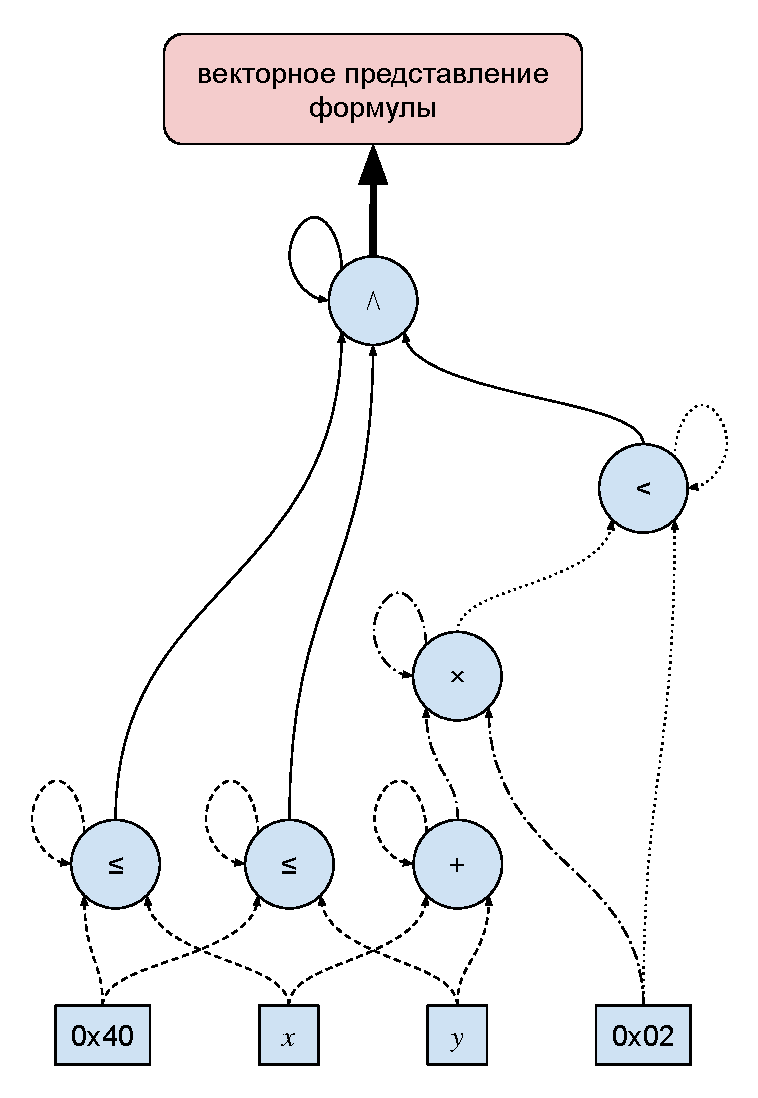
\includegraphics[scale=0.95]{./assets/formula-ast-message-flow.pdf}
    \caption{\label{formula-ast-message-flow} Пример ориентированного ациклического графа, полученного из AST формулы $(\texttt{0x40} \le x) \wedge (\texttt{0x40} \le y) \wedge ((x + y) \times \texttt{0x02} < \texttt{0x02})$ в логике вычислений с восьмибитными векторами. Вершины разбиты по уровням согласно порядку вычислений состояний: снизу истоки (листья) --- с них начинается вычисление, сверху сток (корень) --- его вектор вычисляется последним, и он же считается итоговым вектором-представлением всей формулы. Начертание каждого ребра отражает момент, в который по нему производится передача сообщения: по рёбрам, нарисованным штриховой линией (- - -) передача производится на первом шаге, штрих-пунктирной линией (- $\cdot$ -) --- на втором, пунктирной линией ($\cdot$ $\cdot$ $\cdot$) --- на третьем, а сплошной (\sout{\ \ \ \ \ }) --- на четвёртом. Петли в данном графе обозначают, что для вычисления состояния вершины также используется её начальное состояние (об этом подробнее написано в параграфах про начальные состояния вершин и вычисление их состояний).}
\end{center}
\end{figure}

Описанная выше структура была придумана мной при попытке оптимизировать методы вычислений из статьи \cite{gnn-for-scheduling-paper}, чтобы все нужные состояния можно было посчитать за один проход по AST формулы. Тем не менее, позже, в процессе очередной итерации исследования предметной области, выяснилось, что такая архитектура была придумана ещё в 1997 году, описана в статьях \cite{rvnn-intro-paper} и \cite{rvnn-intro-paper-2} и более известна как рекурсивная нейронная сеть или RvNN\footnote{От англ. \textit{Recursive Neural Network}.}. Авторы указанных статей пытались изобрести подход к обучению моделей для иерархически устроенных данных (рис.~\ref{rvnn-data-tree}), чтобы можно было учитывать и их специфику наряду с тем, как это происходит в свёрточных сетях для данных в виде картинок или в рекуррентных сетях для данных в виде последовательностей. В итоге, было предложено использовать процедуру, похожую на передачу сообщений в GNN, применительно к дереву или ориентированному ациклическому графу, задающим саму иерархию в данных. В статье даже в качестве одного из примеров таких данных рассматриваются логические термы (рис.~\ref{rvnn-term-dag}).

\begin{figure}[!ht]
\begin{center}
    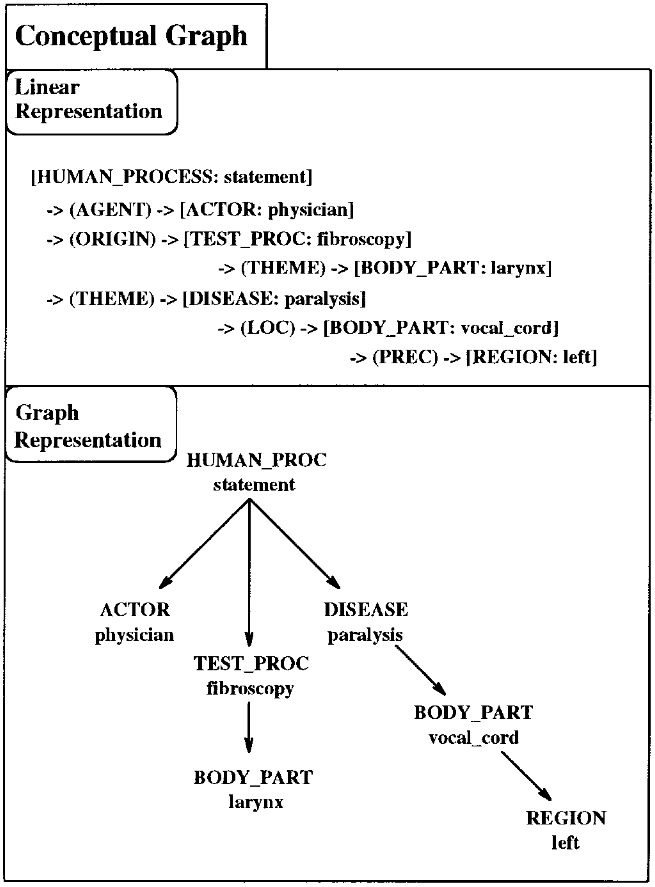
\includegraphics[scale=0.45]{./assets/rvnn-data-tree.png}
    \caption{\label{rvnn-data-tree} Пример иерархически устроенных данных: анамнез пациента. Картинка взята из статьи \cite{rvnn-intro-paper}.}
\end{center}

\begin{center}
    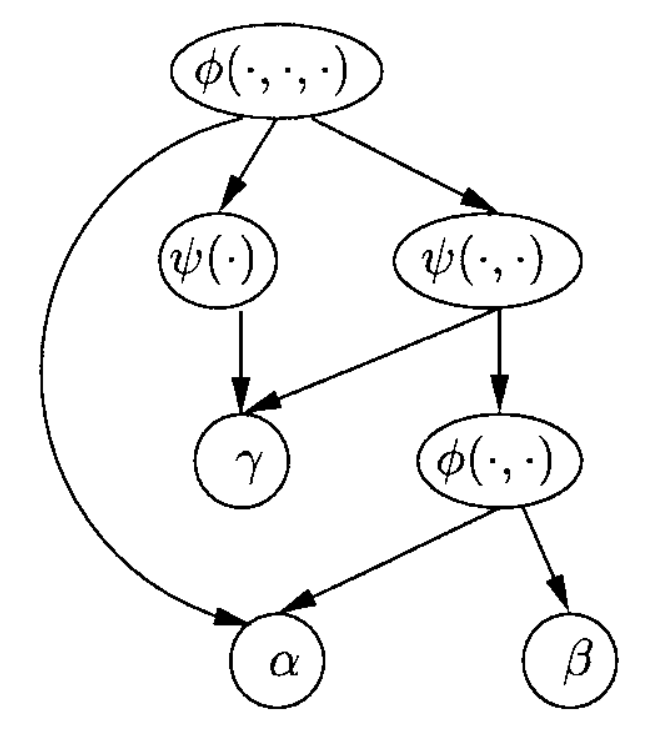
\includegraphics[scale=0.2]{./assets/rvnn-term-dag.png}
    \caption{\label{rvnn-term-dag} Пример представления логического терма $\phi(\alpha, \psi(\gamma), \psi(\gamma, \phi(\alpha, \beta)))$ в виде ориентированного ациклического графа. Картинка взята из статьи \cite{rvnn-intro-paper-2}.}
\end{center}
\end{figure}

Однако с ростом доступных вычислительных мощностей данный подход уступил более обобщённому подходу с использованием GNN и не получил активного дальнейшего развития.

Посчитанный в ходе описанных выше действий вектор-представление графа считается эмбеддингом формулы, который потом можно передать в MLP для предсказания различных параметров формулы, например, её выполнимости. Именно так делается у меня, и ровно так же было предложено делать в статье \cite{rvnn-intro-paper} (рис.~\ref{rvnn-process}).

\begin{figure}[ht]
\begin{center}
    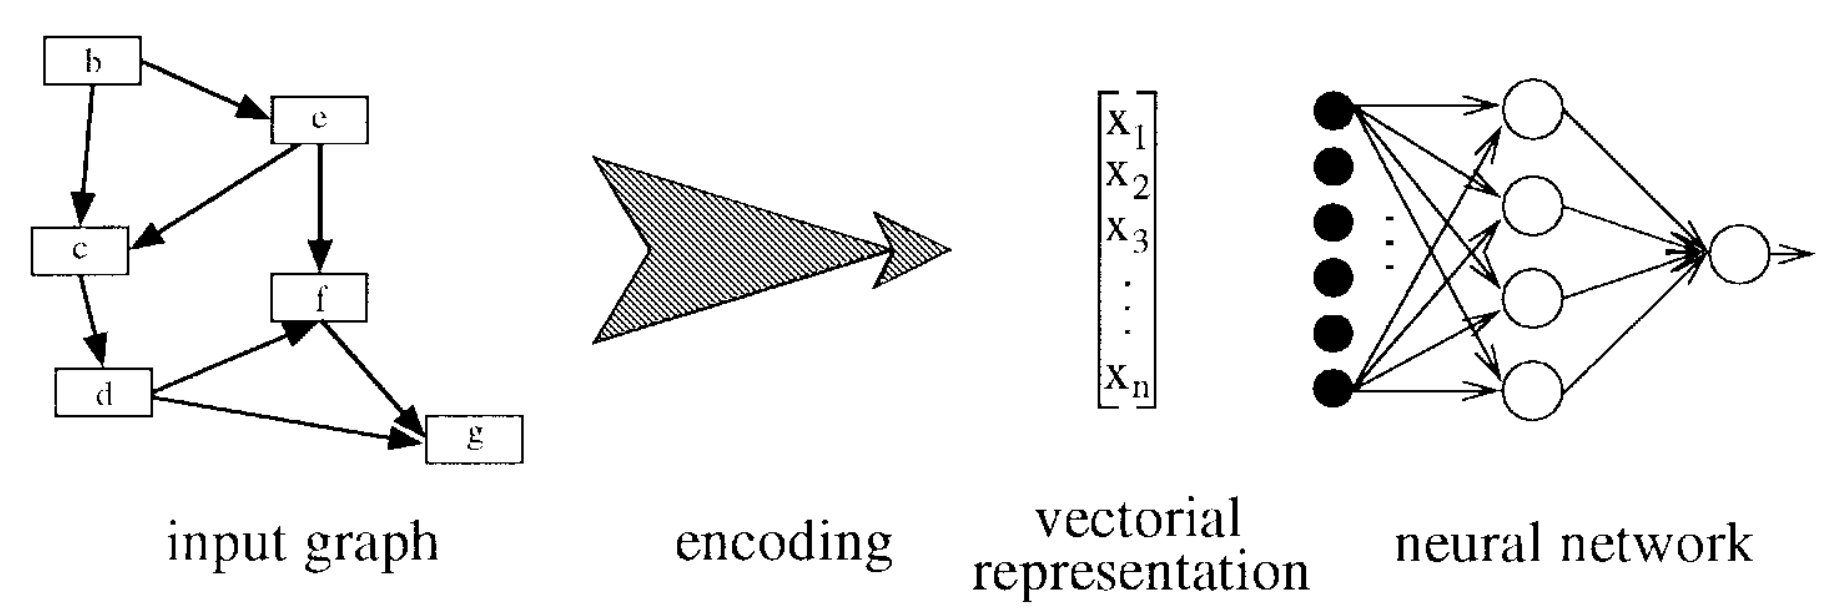
\includegraphics[scale=0.25]{./assets/rvnn-process.png}
    \caption{\label{rvnn-process} Общий подход к решению задачи предсказания произвольных параметров ориентированного ациклического графа. Картинка взята из статьи \cite{rvnn-intro-paper}.}
\end{center}
\end{figure}

\subsection{Начальные состояния вершин} \label{vertex-initial-states}

Выше написано, что в вычислениях участвуют начальные векторы-состояния вершин, но до этого момента не было сказано, откуда они берутся.

С начальными векторами вершин-операций всё легко: эмбеддинг для каждой из них просто выучивается, как это делается, например, для слов в задаче обработки естественного языка, и сохраняются в специальную таблицу. Замечу, что на этом этапе можно сделать разделение одной операции, работающей с разными типами данных, на разные, чтобы учесть отличия в механизме их работы. Например, сложение целых чисел, сложение вещественных чисел и сложение битовых векторов можно считать разными операциями.

С начальными векторами вершин-переменных и вершин-констант всё куда сложнее. Начальный вектор для вершины-переменной должен содержать некоторую информацию о том, что эта вершина соответствует переменной определённого типа, однако с этим есть несколько проблем. Во-первых, векторы, кодирующие разные переменные должны отличаться друг от друга, чтобы как-то отразить то, что в выполняющем наборе формулы им могут быть присвоены разные значения. Во-вторых, эти векторы нельзя основывать на информации об именах переменных, поскольку обычно имя переменной не несёт в себе никакого смысла и используется для разделения переменных внутри одной формулы, да и сами логические формулы инвариантны относительно переименования переменных.

В процессе работы было придумано три возможных варианта действий с переменными:

\begin{enumerate}
    \item Можно проигнорировать все имена переменных в формуле, оставив только информацию об их типе. После такого преобразования все переменные можно считать конструкциями вида \texttt{Var[Тип]}, поэтому в формуле вместо имён переменных будут записи \texttt{Var[Integer]}, \texttt{Var[Real]}, \texttt{Var[BitVec<8>]}, \texttt{Var[Array<BitVec<12>, Float64>]} и прочие подобные. Таких записей будет немного, поэтому для них можно выучить эмбеддинги подобно тому, как это делается для вершин-операций. Такой подход не учитывает различия между переменными, однако позволяет представить формулу в хоть каком-нибудь виде. Например, в формуле на рис.~\ref{formula-ast-message-flow} у переменных $x$ и $y$ будет одинаковое начальное состояние, соответствующее эмбеддингу, выученному для записи \texttt{Var[BitVec<8>]}.
    \item Можно завести отдельную табличку с набором эмбеддингов для переменных и на каждом запуске модели при обучении или при использовании выдавать каждой переменной случайный эмбеддинг из этого набора. Такая схема будет предоставлять разные векторы разным переменным и не будет привязывать их к именам этих переменных, чтобы учесть свойство инвариантности формул относительно переименования. Предполагается, что процессе обучения векторы будут сходиться к случайным точкам, которые достаточно хорошо описывают семантику переменных, а модель научится определённым образом подстраиваться под эту случайность. Это даже можно считать способом регуляризацией модели.
    \item Помимо этого, можно сделать так же, как в предыдущем пункте, но не выучивать табличку с эмбеддингами, а вместо этого случайным образом нумеровать переменные натуральными числами, после чего для этих номеров применять технику позиционного кодирования (англ. \textit{positional encoding}) из знаменитой статьи <<Attention Is All You Need>> \cite{attention-is-all-you-need}. Идея работает такая же, как и пункт 2, но имеет меньше обучаемых параметров и потенциально лучше обобщается на формулы большого размера.
\end{enumerate}

Если про технику работы с переменными всё более-менее понятно (хотя бы понятно, в каком направлении развивать решение), то константы в формуле представляют настоящую проблему, так как нужно научиться переводить и целые числа, и вещественные числа, и битовые векторы, и массивы значений в некоторое многомерное пространство с сохранением всей семантики: абсолютных значений, отношений больше-меньше, внутренней структуры (для битовых векторов и массивов). Задача построения такого представления оказалась слишком сложной, и за время работы не было придумано никаких методов, которые, в теории, могли бы дать существенный прирост качества. Тем не менее, здесь также можно выписать три варианта, что можно сделать с кодированием констант:

\begin{enumerate}
    \item Можно поступить аналогично первому варианту подхода к переменным --- убрать значения всех констант и оставить вместо них только конструкции вида \texttt{Val[Тип]}, после чего обучать эмбеддинги для этих конструкций. Например, в формуле на рис.~\ref{formula-ast-message-flow} у значений \texttt{0x02} и \texttt{0x40} будет одинаковое начальное состояние, соответствующее эмбеддингу, выученному для записи \texttt{Val[BitVec<8>]}.
    \item Можно воспользоваться способом, предложенным в статье \cite{embeddings-for-numerical-features-paper} --- разбивать пространство значений, из которого приходит константа (например, для вещественной переменной это будет вещественная прямая), на группы (бины) и строить вектор, как это показано на рис.~\ref{linear-bins-for-values}. Такой способ, к сожалению, не применим для битовых векторов, так как они могут иметь произвольный размер, а без априорного знания про этот размер отобразить вектор в линейное пространство с сохранением семантики всех операций невозможно.
    \item Помимо этого, можно воспользоваться техникой под названием Fourier Feature Mapping \cite{ffm-paper-1} \cite{ffm-paper-2} --- вторым способом, предложенным в статье \cite{embeddings-for-numerical-features-paper}. Эта статья исследует способы кодирования семантики произвольных числовых значений и ставит своей целью приблизить нейронные сети к градиентным бустингам по качеству решения задач табличного машинного обучения. Насколько я понял, техника заключается в вычислении некоторого количества дискретных преобразований Фурье с разными частотами и использовании полученных значений в качестве координат вектора-эмбеддинга.
\end{enumerate}

\begin{figure}[ht]
\begin{center}
    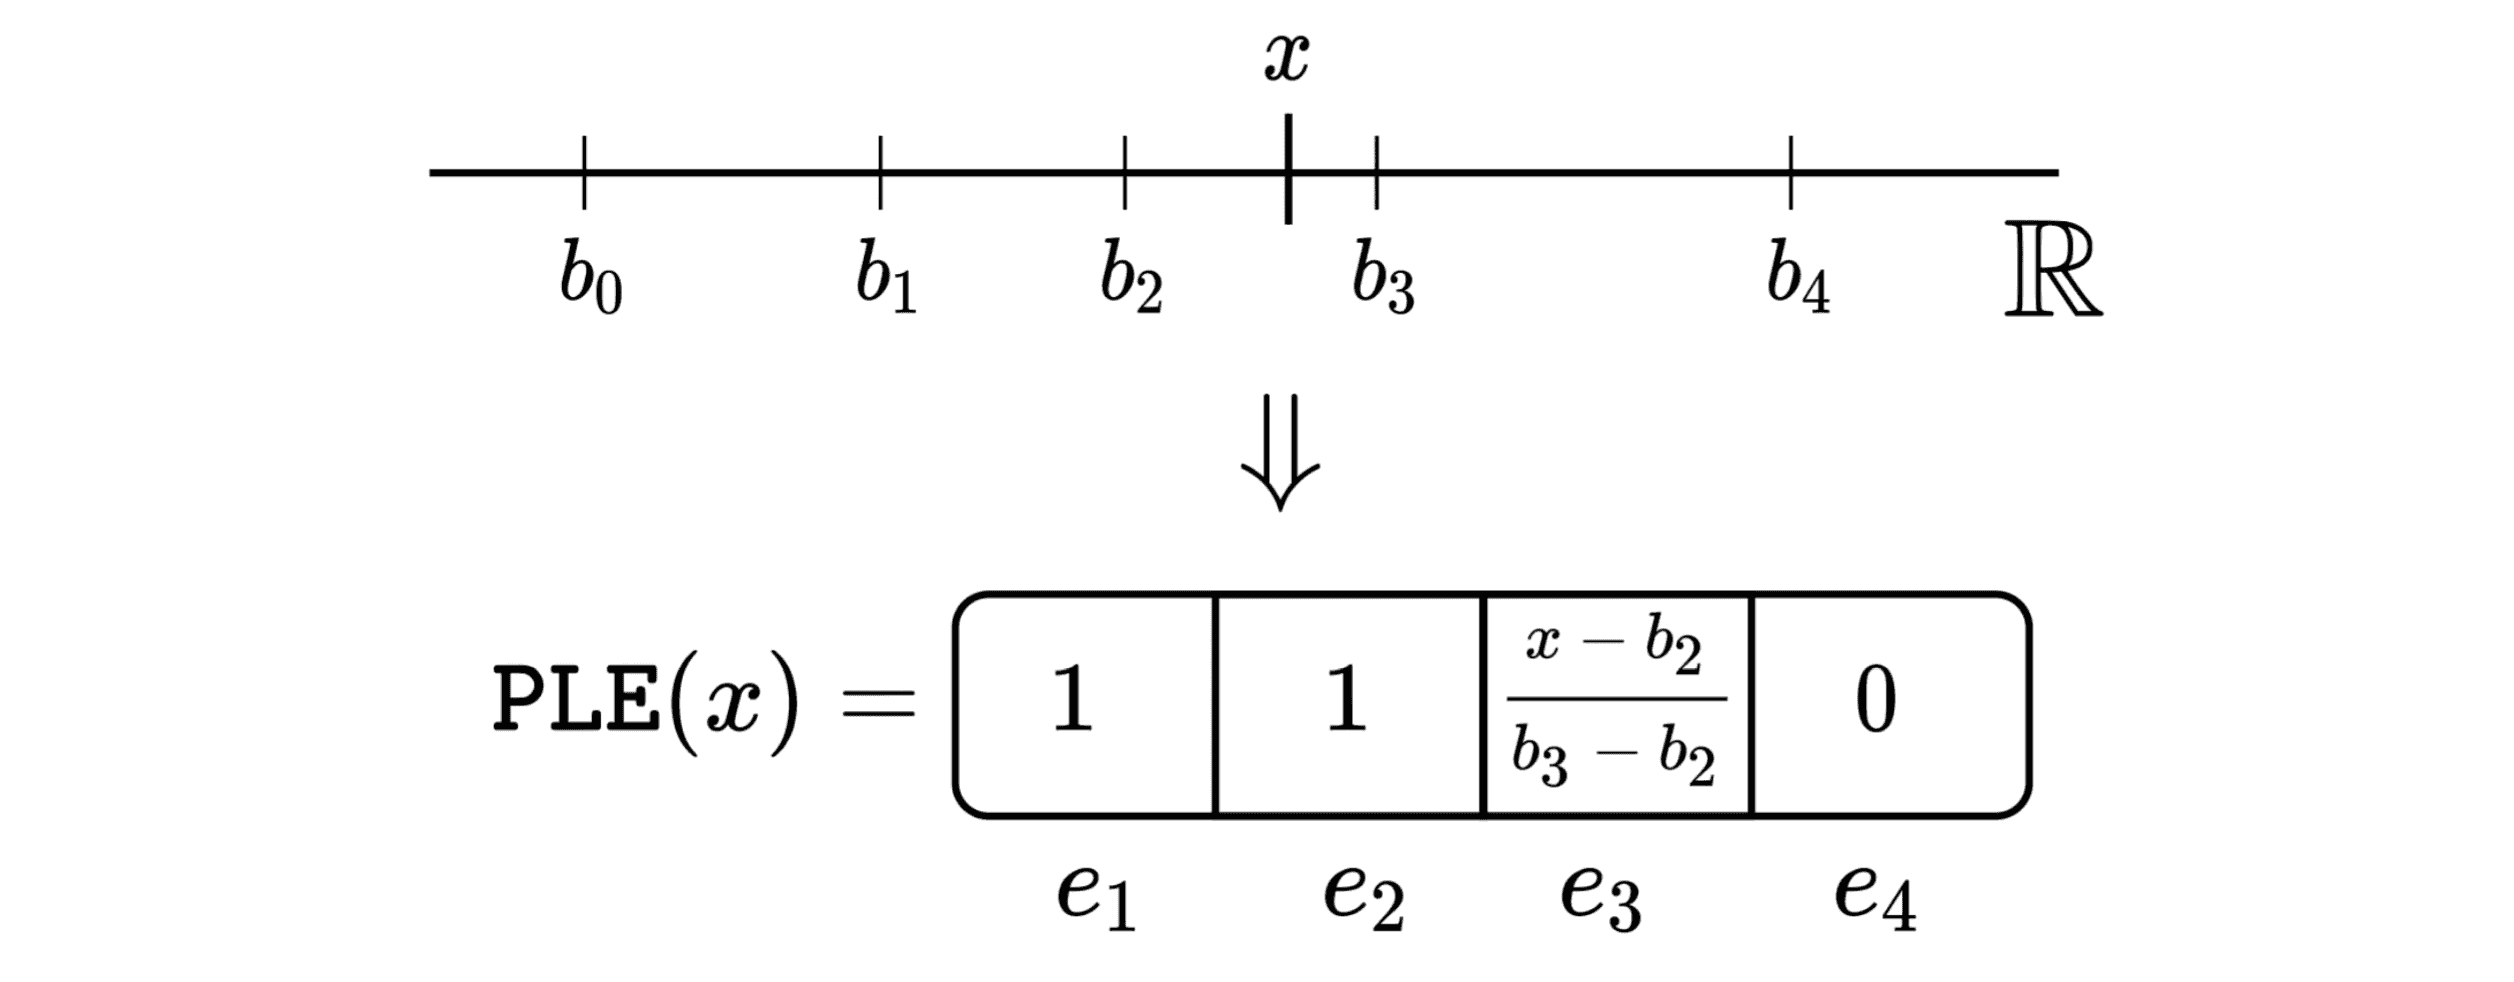
\includegraphics[scale=0.25]{./assets/linear-bins-for-values.png}
    \caption{\label{linear-bins-for-values} Построение эмбеддинга вещественной константы с помощью бинов. Картинка взята из статьи \cite{embeddings-for-numerical-features-paper}.}
\end{center}
\end{figure}

\subsection{Вычисление состояний вершин}

Теперь пришло время поговорить про то, каким способом, собственно, вычислять вектор-состояние очередной вершины. Согласно схеме обновления состояний в GNN это должно происходить посредством передачи векторов-сообщений от соседних вершин. Осталось только выбрать, какие функции подставить в формулу~(\ref{gnn-state-update-rule}). В экспериментах участвовали два варианта.

\subsubsection{SAGE Convolution} \label{sage-conv-desc}

Первый был представлен в статье \cite{sage-conv-paper} и называется GraphSAGE. В нём вычисление происходит согласно формуле~(\ref{sage-conv-update-formula}), где $x_v$ --- изначальное состояние вершины $v$, а $x_v'$ --- новое, которое вычисляется в процессе.

\begin{equation} \label{sage-conv-update-formula}
    x_v' = \sigma \left(W_3 \cdot \left(W_1 \cdot x_v + W_2 \cdot \underset{u \in \mathcal{N}(v)}{\text{\textsc{mean}}} x_u \right) + b \right)
\end{equation}

Здесь $\mathcal{N}(v)$ --- окрестность вершины $v$, функция \textsc{mean} обозначает взятие среднего значения по указанному множеству, $\sigma$ --- сигмоидная функция\footnote{$\sigma(x) = \dfrac{1}{1 + e^{-x}}$}, а матрицы $W_1$, $W_2$, $W_3$ и вектор $b$ являются выучиваемыми параметрами сети.

\subsubsection{Transformer Convolution} \label{transformer-conv-desc}

Второй подход был представлен в статье \cite{transformer-conv-paper} и называется Transformer Graph Convolution. В нём вычисление происходит согласно формулам (\ref{transformer-conv-update-formula-att-coefs}) и (\ref{transformer-conv-update-formula}).

\begin{equation} \label{transformer-conv-update-formula-att-coefs}
    \alpha_{u} = \underset{u \in \mathcal{N}(v)}{\text{\textsc{softmax}}} \left[\frac{(W_3 \cdot x_v)^T (W_4 \cdot x_u)}{\sqrt d} \right]
\end{equation}

\begin{equation} \label{transformer-conv-update-formula}
    x_v' = W_1 \cdot x_v + \sum_{u \in \mathcal{N}(v)} \alpha_u W_2 \cdot x_u
\end{equation}

Здесь $d$ --- размерность участвующих в вычислениях векторов, функция \textsc{softmax} по указанному множеству обозначает softmax-преобразование\footnote{$\text{\textsc{softmax}}(a_1, a_2, \ldots, a_n)_k = \dfrac{e^{a_k}}{\sum \limits_{i = 1}^n e^{a_i}}$} чисел этого множества, а матрицы $W_1$, $W_2$, $W_3$ и $W_4$ являются выучиваемыми параметрами сети.

Нетрудно заметить, что механизм вычислений похож на тот, что используется в архитектуре Transformer \cite{attention-is-all-you-need} (собственно, оттуда и название подхода): значения $\alpha$ являются коэффициентами механизма внимания, матрица $W_3$ формирует вектор-запрос, $W_4$ --- вектор-ключ, а $W_2$ --- вектор-значение.

\subsubsection{Учёт начального состояния вершины}

Из формул (\ref{sage-conv-update-formula}) и (\ref{transformer-conv-update-formula}) видно, что для вычисления вектора-состояния вершины используется её же начальное состояние (в указанных формулах оно домножается на матрицу $W_1$). Именно таким образом и происходит учёт информации об операции, которой соответствует вершина: изначально в вершину кладётся вектор, представляющий семантику этой операции, а потом он используется при вычислении состояния этой вершины через состояния её детей. Петли в графе на рис.~\ref{formula-ast-message-flow} обозначают в точности это.

\subsection{Классификатор и функция потерь}

С точки зрения нейронной сети задача поставлена как задача классификации, поэтому после прохода по графу и вычисления всех состояний вектор-состояние корневой вершины отправляется в классификатор, который представляет из себя нейронную сеть с четырьмя полносвязными слоями и слоями активации ReLU между ними.

В качестве функции потерь используется бинарная кросс-энтропия.

\newpage

\section{Эксперименты и результаты}

% todo: тут в основной части можно красивый барплот, а в приложении огромную таблицу

К сожалению, из-за присутствовавших трудностей с вычислительными мощностями все эксперименты проводились с использованием векторов-состояний вершин размера исключительно 32 (другие размеры попробовать не удалось), а из описанных в разделе~\ref{vertex-initial-states} методов построения начальных состояний вершин были попробованы только первые методы построения состояний для переменных и констант. Однако, даже с такими подходами удалось провести ряд экспериментов и получить некоторые практически значимые результаты.

\subsection{Первый эксперимент}

В первом эксперименте была предпринята попытка обучить модель с архитектурой SAGE Convolution, описанной в разделе~\ref{sage-conv-desc}, на датасетах из формул с SMT-COMP (таблица~\ref{smt-comp-datasets-table}).

Для полноты картины эксперимент был устроен следующим образом: было обучено три модели (по одной на каждом из датасетов), после чего для каждой полученной модели считались метрики на её обучающем датасете, на его частных случаях (например, \texttt{BitVec} $\subset$ \texttt{SymbEx}) или на его альтернативных вариантах (например, для \texttt{SymbEx} был взят датасет \texttt{usvm-test}, из формул, собранных с символьной машины \cite{usvm-diploma}). Это сделано, чтобы, в том числе, узнать, может ли знание о более сложных формулах помочь модели разбираться с более простыми.

Разумеется, в случае, когда модель обучалась на датасете \texttt{X}, подсчёт метрик на этом датасете производится на специально отложенной тестовой выборке\footnote{В этом и во всех последующих экспериментах в каждом датасете примерно 15\% формул были отложены в валидационную выборку, и ещё примерно 10\% --- в тестовую.}. Если датасет \texttt{X} не участвовал в обучении модели, то метрики считались на всех его данных. Это соблюдается в этом и во всех последующих экспериментах.

Обучение каждой модели производилось в течение 50 эпох с помощью оптимизатора Adam \cite{adam-paper} с learning rate\footnote{Так называют длину шага градиентного спуска.}, изначально равным $10^{-4}$, и управляемым согласно динамическому расписанию \textit{Reduce LR On Plateau}.

В течение всего обучения проводился отбор лучших моделей (англ. \textit{model selection}) по значению функции потерь на валидационной выборке.

Результаты отображены в таблице~\ref{smt-comp-val-results}. К сожалению, они получились не особо впечатляющими --- во время обучения даже на тренировочном датасете функция потерь упиралась в границу, которую никак не могла преодолеть, так что модель выглядит недообученной. Оно и понятно --- модель не умеет отличать переменные друг от друга и не понимает семантику констант в формуле.

\begin{table}[ht]
\begin{center}
\begin{tabular}{c|c||cc|cc}
    \makecell{Трен. \\ датасет} & \makecell{Вал. \\ датасет} & \makecell{Контр-ный \\ \textsc{ROC-AUC}} & \makecell{Тестовый \\ \textsc{ROC-AUC}} & \makecell{Контр-ный \\ \textsc{AP}} & \makecell{Тестовый \\ \textsc{AP}} \\
    \hline \hline
    \rule{0pt}{2.5ex}
    \texttt{BitVec}  & \texttt{BitVec}     & 0.500 & 0.718 & 0.378 & 0.695 \\
    \hline
    \texttt{SymbEx}  & \texttt{BitVec}     & 0.500 & 0.548 & 0.378 & 0.426 \\
                     & \texttt{SymbEx}     & 0.500 & 0.358 & 0.610 & 0.678 \\
                     & \texttt{usvm-test}  & 0.500 & 0.503 & 0.038 & 0.054 \\
    \hline
    \texttt{QuaFree} & \texttt{BitVec}     & 0.500 & 0.719 & 0.378 & 0.706 \\
                     & \texttt{SymbEx}     & 0.500 & 0.592 & 0.610 & 0.716 \\
                     & \texttt{QuaFree}    & 0.500 & 0.564 & 0.622 & 0.705 \\
\end{tabular}
\caption{\label{smt-comp-val-results} Метрики, полученные при обучении SAGE Convolution на датасетах с SMT-COMP \cite{smt-comp-2023-benchmarks}.}
\end{center}
\end{table}

\subsection{Второй эксперимент}

Второй эксперимент заключался в обучении модели с той же архитектурой, что и в первом эксперименте, но уже на других датасетах. В этот раз были рассмотрены датасеты из формул, собранных с символьного движка USVM \cite{usvm-diploma} (таблица~\ref{usvm-train-datasets-table}).

Аналогично первому эксперименту, здесь модель обучалась на каком-то датасете, после чего валидировалась, в том числе, на некоторых других датасетах, однако на этот раз валидационные датасеты, в основном, не пересекались с тренировочными. Сделано это было, чтобы можно было оценить обобщающую способность модели. Подробнее об этом было написано во втором абзаце раздела~\ref{usvm-datasets-desc}.

Обучение каждой модели производилось в течение 30 эпох с помощью оптимизатора AdamW \cite{adamw-paper} с параметром weight decay\footnote{Параметр отвечает за регуляризацию модели на основе штрафа за слишком большие абсолютные значения весов.}, равным $10^{-3}$, и learning rate, изначально равным $10^{-4}$, и управляемым согласно динамическому расписанию \textit{Reduce LR On Plateau}. Такое большое значение weight decay было продиктовано желанием как можно сильнее повысить обобщающую способность модели, чтобы она потенциально могла показывать хорошее качество на данных из другого распределения.

В течение всего обучения проводился отбор лучших моделей по значению функции потерь на валидационной выборке.

Результаты в таблице~\ref{usvm-train-ds-val-results}.

\begin{table}[ht]
\begin{center}
\begin{tabular}{c|c||cc|cc}
    \makecell{Трен. \\ датасет} & \makecell{Вал. \\ датасет} & \makecell{К. \\ \textsc{ROC-AUC}} & \makecell{Т. \\ \textsc{ROC-AUC}} & \makecell{К. \\ \textsc{AP}} & \makecell{Т. \\ \textsc{AP}} \\
    \hline \hline
    \rule{0pt}{2.5ex}
    \texttt{usvm-test} & \texttt{usvm-test}      & 0.500 & 0.873 & 0.038 & 0.566 \\
    \cline{2-6}
    \rule{0pt}{2.5ex}
                       & \texttt{the-algorithms} & 0.500 & 0.551 & 0.066 & 0.067 \\
    \cline{2-6}
    \rule{0pt}{2.5ex}
                       & \texttt{usvm-core}      & 0.500 & 0.641 & 0.066 & 0.087 \\
    \cline{2-6}
    \rule{0pt}{2.5ex}
                       & \texttt{owasp-all}      & 0.500 & 0.314 & 0.029 & 0.101 \\
    \hline
    \makecell{
        \texttt{usvm-test} \& \\
        \texttt{the-algorithms}
    } & \makecell{
        \texttt{usvm-test} \& \\
        \texttt{the-algorithms}
    }                      & 0.500 & 0.786 & 0.053 & 0.447 \\
    \cline{2-6}
    \rule{0pt}{2.5ex}
      & \texttt{usvm-core} & 0.500 & 0.833 & 0.066 & 0.198 \\
    \cline{2-6}
    \rule{0pt}{2.5ex}
      & \texttt{owasp-all} & 0.500 & 0.636 & 0.029 & 0.260 \\
    \hline
    \makecell{
        \texttt{usvm-test} \& \\
        \texttt{the-algorithms} \& \\
        \texttt{usvm-core}
    } & \makecell{
        \texttt{usvm-test} \& \\
        \texttt{the-algorithms} \& \\
        \texttt{usvm-core}
    }                      & 0.500 & 0.821 & 0.058 & 0.593 \\
    \cline{2-6}
    \rule{0pt}{2.5ex}
      & \texttt{owasp-all} & 0.500 & 0.958 & 0.029 & 0.873 \\
\end{tabular}
\caption{\label{usvm-train-ds-val-results} Метрики, полученные при обучении SAGE Convolution на датасетах, собранных с USVM \cite{usvm-diploma}. Символ <<\&>> здесь обозначает объединение датасетов. <<К.>> обозначает контрольное значение, <<Т.>> --- тестовое.}
\end{center}
\end{table}

Здесь метрики выглядят куда интереснее, чем в первом эксперименте. Во-первых, полученные числа сами по себе выглядят более солидно. Во-вторых, хорошо видно, как растёт обобщающая способность модели, если обучать её на более сложных и разнообразных формулах. Особенно, это заметно по метрикам на датасете \texttt{owasp-all} (версия датасета \texttt{owasp}, из которой не убирали формулы слишком маленького размера).

\subsection{Третий эксперимент}

Удачные результаты второго эксперимента (особенно полученные на датасете \texttt{owasp-all}) натолкнули на мысль, что, возможно, последняя обученная модель (нижняя в таблице~\ref{usvm-train-ds-val-results}) уже достаточно хороша, чтобы уметь предсказывать ответ для формул, возникающих в процессе анализа \textit{произвольных} программ с помощью символьного движка USVM.

Для проверки этой гипотезы были собраны датасеты из формул, возникших в процессе анализа разных проектов с открытым исходным кодом, написанных на JVM-языках (таблица~\ref{usvm-val-datasets-table}), и на них были посчитаны уже знакомые нам метрики. Результаты в таблице~\ref{usvm-val-results-roc-auc-avg-prec}.

\begin{table}[ht]
\begin{center}
\begin{tabular}{r|cc|cc}
    Датасет & \makecell{Контрольный \\ \textsc{ROC-AUC}} & \makecell{Тестовый \\ \textsc{ROC-AUC}} & \makecell{Контрольный \\ \textsc{AP}} & \makecell{Тестовый \\ \textsc{AP}} \\
    \hline \hline
    \rule{0pt}{2.5ex}
    \texttt{BitVec}           & 0.500 & 0.613 & 0.378 & 0.484 \\
    \texttt{SymbEx}           & 0.500 & 0.509 & 0.610 & 0.628 \\
    \hline
    \texttt{owasp}            & 0.500 & 0.914 & 0.029 & 0.245 \\
    \texttt{cassandra}        & 0.500 & 0.956 & 0.057 & 0.603 \\
    \texttt{kafka}            & 0.500 & 0.827 & 0.083 & 0.689 \\
    \texttt{spark-core}       & 0.500 & 0.970 & 0.061 & 0.616 \\
    \texttt{spark-streaming}  & 0.500 & 0.992 & 0.057 & 0.889 \\
    \texttt{utbot-core}       & 0.500 & 0.982 & 0.061 & 0.657 \\
    \texttt{utbot-java}       & 0.500 & 0.997 & 0.045 & 0.911 \\
    \texttt{utbot-python}     & 0.500 & 0.923 & 0.115 & 0.480 \\
    \texttt{utbot-js}         & 0.500 & 0.801 & 0.062 & 0.307 \\
    \texttt{utbot-go}         & 0.500 & 0.996 & 0.014 & 0.712 \\
    \texttt{zookeeper}        & 0.500 & 0.840 & 0.046 & 0.407 \\
    \texttt{elasticsearch}    & 0.500 & 0.999 & 0.001 & 0.468 \\
    \texttt{hbase}            & 0.500 & 0.824 & 0.019 & 0.083 \\
    \texttt{guava}            & 0.500 & 0.998 & 0.014 & 0.816 \\
    \texttt{hadoop-common}    & 0.500 & 0.975 & 0.081 & 0.714 \\
    \texttt{hadoop-hdfs}      & 0.500 & 0.847 & 0.032 & 0.379 \\
    \texttt{hadoop-mapreduce} & 0.500 & 0.948 & 0.011 & 0.198 \\
    \texttt{hadoop-yarn}      & 0.500 & 0.994 & 0.035 & 0.845 \\
\end{tabular}
\caption{\label{usvm-val-results-roc-auc-avg-prec} Результаты валидации на датасетах из реальных формул, собранных с символьной машины USVM \cite{usvm-diploma} (см. таб.~\ref{usvm-val-datasets-table}).}
\end{center}
\end{table}

Думаю, что результаты достаточно хороши, для того, чтобы их можно было считать в значительной степени положительными, и чтобы полученную модель можно было использовать на практике.

Поскольку обычно в процессе символьного исполнения распознавание выполнимых формул важнее, чем распознавание невыполнимых, я также привожу результаты метрик <<precision @ fixed recall>> (уровень точности при заданном уровне полноты) в таблице~\ref{usvm-val-results-precs-at-recall} в приложении.

Тем не менее, видно, что результаты на датасетах \texttt{BitVec} и \texttt{SymbEx} с SMT-COMP (таблица~\ref{smt-comp-datasets-table}), в которых содержатся формулы из аналогичных логик, оставляют желать лучшего. Так что, скорее всего, высокие результаты на оставшихся датасетах обусловлены, в первую очередь, тем, что в процессе работы движка USVM получаются сильно специфические формулы, по структуре которых легко предсказать их выполнимость. Однако, это не повод не использовать данную особенность при решении практической задачи.

\subsection{Четвёртый эксперимент}

Для полноты исследования было также решено попробовать обучить модель с другой архитектурой (Transformer Convolution из раздела~\ref{transformer-conv-desc}), однако этот эксперимент оказался неудачным.

При обучении на датасетах с SMT-COMP (таблица~\ref{smt-comp-datasets-table}) где-то после седьмой-восьмой эпохи модель начинала бесконтрольно переобучаться (метрики на тренировочном наборе уверенно улучшались, а на валидационном стремительно ухудшались). Причём лучшая модель, полученная на тот момент, всё равно проигрывала модели с архитектурой SAGE Convolution.

Более того, в архитектуру Transformer Convolution встроена возможность использовать механизм dropout \cite{dropout-paper} при обучении, и подобная проблема проявлялась даже при вероятности отключения нейрона $p = 0.2, \ 0.3, \ 0.4, \ 0.5$. Использование техники Layer Normalization \cite{layer-norm-paper}, которая часто помогает при проблемах с обучением механизма внимания, тоже не дало улучшений.

Видимо, действительно, данные в датасетах с SMT-COMP устроены настолько сложно и отражают настолько общий случай, что никакие техники, успешно показывающие себя на датасетах с USVM (раздел~\ref{usvm-datasets-desc}), здесь не работают.

Сами датасеты, собранные с USVM, в этом эксперименте не использовались, и качество на них не измерялось, поскольку модель с такой архитектурой будет иметь значительные проблемы с производительностью, поэтому получение прироста качества за счёт перехода на такую архитектуру на практике может обернуться замедлением работы всей системы и, как следствие, оказаться бесполезным.

\newpage

\section{Дальнейшее развитие} \label{future-works}

Несмотря на неплохие результаты на некоторых имеющихся датасетах, модель можно улучшить во многих местах. Вот список направлений, по которым стоит развивать проект:

\begin{enumerate}
    \item Попробовать провести эксперименты с разными гиперпараметрами нейронной сети: попробовать другие (отличные от 32) значения размерности вектора-состояния вершины, другое количество линейных слоёв в классификаторе и т. д..
    \item Разумеется, стоит попробовать использовать более содержательные из описанных в разделе~\ref{vertex-initial-states} техник построения векторного представления переменных и констант в формуле.
    \item Можно запускать передачу сообщений по графу формулы не только в одном направлении, а сразу во всех, как это было сделано в статье \cite{gnn-for-scheduling-paper}, а после этого использовать не только состояние корневой вершины, а агрегировать информацию сразу со всех вершин.
    \item Чтобы увеличить датасет и повысить обобщающую способность модели, можно попробовать применить разного рода аугментации к формулам в тренировочном датасете.
    \item Если получится научиться проверять на выполнимость относительно произвольные формулы, можно озаботиться поддержкой формул с кванторами.
    \item Поскольку использование модели на практике предполагает не столько предсказательную способность модели, сколько ранжирующую, можно попробовать применить техники из этой области. Например: учитывать косинусное расстояние между вычисляемыми векторами, представляющими выполнимые и невыполнимые формулы, использовать ранжирующую функцию потерь LambdaRank \cite{lambda-rank-paper} или функцию потерь Triplet Loss для задач информационного поиска \cite{triplet-loss-paper-1} \cite{triplet-loss-paper-2}.
    \item Нынешняя версия модели не использует имена переменных, считая, что они ничего толкового не значат. Тем не менее, если речь идёт о модели, используемой для распознавания формул, которые возникают при работе USVM, можно попробовать учитывать имена некоторых переменных, так как они порождаются определённым образом, и в них может содержаться какая-то полезная информация.
    \item Если говорить об использовании модели на практике, стоит отметить необходимость её эффективной реализации. Текущая версия модели написана на языках Python и Kotlin и значительно уступает современным SMT-решателям, написанным на языке C++. Помимо этого можно применить различные техники оптимизации вычислений в нейронных сетях как, например, квантизация.
    \item Наконец, после получения быстрой, показывающей хорошее качество на практике модели, можно озаботиться встраиванием её в работу символьного движка USVM \cite{usvm-diploma}. Для этого нужно будет придумать ряд эвристик для выбора состояния, которые будут учитывать предсказание модели. Изначально такая задача не предполагалась, но она является естественным и логичным продолжением исследования, проведённого в этой работе.
\end{enumerate}


\specialsection{Заключение}

Заключение должно подводить итоги работы и содержать информацию о полученных в рамках работы результатах.


% Аргумент {1} ниже включает переопределенный стиль с выравниванием слева
\begin{thebibliography}{1}

\bibitem{smt-logics-picture} SMT-LIB 2 Logics. URL: \url{https://smt-lib.org/logics.shtml} (дата обр. 13.05.2024).

\bibitem{z3-paper} Leonardo de Moura and Nikolaj Bjørner. <<Z3: an efficient SMT solver>>. In proceedings of \textit{Tools and Algorithms for the Construction and Analysis of Systems} (TACAS '2008), pp. 337--340. Springer, 2008.

\bibitem{cvc5-paper} Haniel Barbosa, Clark W. Barrett, Martin Brain, Gereon Kremer, Hanna Lachnitt, Makai Mann, Abdalrhman Mohamed, Mudathir Mohamed, Aina Niemetz, Andres N{\"{o}}tzli, Alex Ozdemir, Mathias Preiner, Andrew Reynolds, Ying Sheng, Cesare Tinelli and Yoni Zohar; Dana Fisman (ed.) and Grigore Rosu (ed.). <<cvc5: {A} Versatile and Industrial-Strength {SMT} Solver>>. In proceedings of \textit{Tools and Algorithms for the Construction and Analysis of Systems} (TACAS '2022), part~{I}, pp. 415--442. Springer, 2022.

\bibitem{yices2-paper} Bruno Dutertre; Armin Biere (ed.) and Roderick Bloem (ed.). <<Yices 2.2>>. In proceedings of \textit{Computer-Aided Verification} (CAV '2014), pp. 737--744. Springer, 2014.

\bibitem{bitwuzla-paper} Aina Niemetz and Mathias Preiner; Constantin Enea (ed.) and Akash Lal (ed.). <<Bitwuzla>>. In proceedings of \textit{Computer-Aided Verification} (CAV '2023), part~{II}, pp. 3--17. Springer, 2023.

\bibitem{smt-comp-paper} Clark Barrett, Leonardo de Moura and Aaron Stump. <<SMT-COMP: Satisfiability modulo theories competition>>. In proceedings of \textit{Computer-Aided Verification} (CAV '2005), pp. 503--516. Springer, 2005.

\bibitem{smt-comp-website} SMT-COMP. URL: \url{https://smt-comp.github.io/} (дата обр. 15.05.2024).

\bibitem{symbex-intro-paper} James C. King. <<Symbolic execution and program testing>>. In \textit{Communications of the ACM}, July 1976, volume 19, number 7, pp. 385--394. Association for Computing Machinery, 1976.

\bibitem{klee-website} KLEE Symbolic Execution Engine. URL: \url{https://klee-se.org/} (дата обр. 15.05.2024).

\bibitem{klee-paper} Cristian Cadar, Daniel Dunbar and Dawson Engler. <<KLEE: Unassisted and Automatic Generation of High-Coverage Tests for Complex Systems Programs>>. In proceedings of \textit{the 8th USENIX conference on Operating systems design and implementation} (OSDI '2008), pp. 209--224. USENIX Association, 2008.

\bibitem{fastsmt-paper} Mislav Balunovic, Pavol Bielik and Martin T. Vechev. <<Learning to Solve SMT Formulas>>. \textit{Advances in Neural Information Processing Systems 31} (2018).

\bibitem{gnn-for-scheduling-paper} Jan H\r{u}la, David Moj\v{z}\'{\i}\v{s}ek and Mikol\'{a}\v{s} Janota. <<Graph Neural Networks for Scheduling of SMT Solvers>>. \textit{IEEE 33rd International Conference on Tools with Artificial Intelligence} (ICTAI '2021), pp. 447--451. IEEE, 2021.

\end{thebibliography}


\end{document}
